\documentclass{IEEEtran}

\usepackage{times}
\usepackage{graphicx}
\usepackage{latexsym}
\usepackage{xspace}
\usepackage{hyperref}
\usepackage{amssymb}
\usepackage{algorithm}
\usepackage[noend]{algpseudocode}
\usepackage[numbers]{natbib}
\usepackage{notoccite}
\usepackage{fixltx2e}
\usepackage{framed}
\usepackage{amsmath}
\usepackage{tabularx}
\usepackage[margin=0.1cm]{subcaption}
\usepackage[inline]{enumitem}

\usepackage[dvipsnames]{xcolor}
\newcommand{\PADSEP}{-7pt}
\newcommand{\sergey}[1]{\textcolor{magenta}{{\sc Sergey:} #1}\xspace}
\newcommand{\samuel}[1]{\textcolor{green}{{\sc Samuel:} #1}\xspace}
\newcommand{\tias}[1]{\textcolor{blue}{{\sc Tias:} #1}\xspace}
\newcommand{\luc}[1]{\textcolor{red}{{\sc Luc:} #1}\xspace}

\newcommand{\constraints}{\ensuremath{\mathcal{T}}\xspace}
\newcommand{\format}[1]{\textit{#1}\xspace}
\newcommand{\generategroups}{\format{SuperblockAssignments}}
\newcommand{\extractgroups}{\format{extractGroups}}
\newcommand{\extracttables}{\format{extractTables}}
\newcommand{\learnconstraints}{\format{LearnConstraints}}
\newcommand{\findassignment}{\format{Subassignments}}
\newcommand{\postprocess}{\format{pruneRedundant}}
\newcommand{\constrainttorder}{\format{templateOrder}}
\newcommand{\template}{\format{constraint template}}
\newcommand{\sname}{\format{TaCLe}}


\newcommand{\CName}{Syntax\xspace}
\newcommand{\CSignature}{Signature\xspace}
\newcommand{\CFunction}{Definition\xspace}
\newcommand{\dependencies}{\ensuremath{\mathcal{D}}\xspace}
\newcommand{\groups}{\ensuremath{\mathcal{B}}\xspace}
\newcommand{\blocks}{\ensuremath{\mathcal{B}}\xspace}

\newcommand{\range}[3]{\ensuremath{#1[#2,#3]}}
\newcommand{\rangeto}[2]{#1{:}#2}
\newcommand{\rangeall}{:}

\newcommand{\eccalc}[2]{\ensuremath{#1 = #2}}
\newcommand{\ecrank}[2]{\eccalc{#1}{\textit{RANK}(#2)}}
\newcommand{\ecfkey}[2]{\ensuremath{\textit{FOREIGNKEY}(#1,#2)}}
\newcommand{\ecalldiff}[1]{\ensuremath{\textit{ALLDIFFERENT}(#1)}}
\newcommand{\eclookupf}[4]{\ensuremath{\textit{LOOKUP}_{\textit{#4}}(#1, #2, #3)}}
\newcommand{\eclookup}[4]{\eccalc{#1}{\eclookupf{#2}{#3}{#4}{}}}
\newcommand{\eclookupprod}[5]{\eccalc{#1}{#2 \times \eclookupf{#3}{#4}{#5}{}}}
\newcommand{\eclookupfuzzy}[4]{\eccalc{#1}{\eclookupf{#2}{#3}{#4}{fuzzy}}}
\newcommand{\ecperm}[1]{\ensuremath{\textit{PERMUTATION}(#1)}}
\newcommand{\ecseries}[1]{\ensuremath{\textit{SERIES}(#1)}}
\newcommand{\ecprod}[3]{\eccalc{#1}{#2 \times #3}}
\newcommand{\ecdiv}[3]{\eccalc{#1}{{#2} / {#3}}}
\newcommand{\ecdiff}[3]{\eccalc{#1}{#2 - #3}}
\newcommand{\ectotal}[3]{\eccalc{#1}{\textit{PREV}(#1) + #2 - #3}}
\newcommand{\ecproj}[2]{\eccalc{#1}{\textit{PROJECT}(#2)}}
\newcommand{\ecaggc}[3]{\eccalc{#2}{\textit{#1\textsubscript{col}}(#3)}}
\newcommand{\ecaggr}[3]{\eccalc{#2}{\textit{#1\textsubscript{row}}(#3)}}
\newcommand{\ecsumc}[2]{\eccalc{#1}{\textit{SUM\textsubscript{col}}(#2)}}
\newcommand{\ecsumr}[2]{\eccalc{#1}{\textit{SUM\textsubscript{row}}(#2)}}
\newcommand{\ecaggif}[5]{\eccalc{#2}{\textit{#1IF}(#3, #4, #5)}}
\newcommand{\ecsumif}[4]{\eccalc{#1}{\textit{SUMIF}(#2, #3, #4)}}
\newcommand{\ecsumprod}[3]{\eccalc{#1}{\textit{SUMPRODUCT}(#2, #3)}}

\newcommand{\numeric}{\format{numeric}}
\newcommand{\textual}{\format{textual}}
\newcommand{\integer}{\format{integer}}
\newcommand{\discrete}{\format{discrete}}
\newcommand{\plength}{\format{length}}
\newcommand{\psize}{\format{size}}
\newcommand{\ptype}{\format{type}}
\newcommand{\ptable}{\format{table}}
\newcommand{\por}{\format{orientation}}
\newcommand{\prows}{\format{rows}}
\newcommand{\pcols}{\format{columns}}
\newcommand{\nat}{\mathcal{N}}

\newcommand{\sg}{B}
\newcommand{\sbl}[1]{\ensuremath{B_{\textit{#1}}}}
\newcommand{\bsbl}[1]{\ensuremath{\mathbf{B_{\textit{#1}}}}}



\renewcommand{\arraystretch}{1.5}

\usepackage{amsthm} % incompatible with ACM
\theoremstyle{definition}
\newtheorem{definition}{Definition}
\newtheorem{example}{Example}
%\newdef{definition}{Definition} % ACM specific


\begin{document}

\title{Learning constraints in spreadsheets and tabular data}
% see http://www.acm.org/binaries/content/assets/publications/article-templates/sig-alternate-sample.tex

%\author{Name1 Surname1 \and Name2 Surname2 \and Name3 Surname3 \institute{----------------------} }

\maketitle

\begin{abstract}
%Spreadsheets, comma separated value files and other tabular data representations are in wide use today. However, the correct use and maintenance of functions in and between the tabular data can be error-prone and overwhelming. In this work, we investigate the automatic discovery of constraints (functions and relations) from raw tabular data. Our method takes inspiration form inductive logic programming and constraint satisfiability. We represent common spreadsheet functions as predicates with arguments that must satisfy number of constraints over the arguments. This allows generic constraint satisfaction techniques to be used to find all such satisfying predicates/functions within the rows, columns and submatrices of the tables. We show the effectiveness and accuracy of this approach on a number of spreadsheets from varying sources.
Spreadsheets, CSV (comma separated value) files and other tabular data representations are in wide use today.
However, modeling, maintaining and discovering formulas in tabular data and spreadsheets can be time consuming and error-prone.
In this work, we investigate the automatic discovery of constraints (functions and relations) from raw tabular data.
We see multiple promising applications for this technique, e.g. in rediscovering constraints, auto-completion and error checking.
Our method takes inspiration from inductive logic programming, constraint learning and constraint satisfaction.
Common spreadsheet functions are represented as predicates whose arguments must satisfy a number of constraints.
Constraint learning techniques are used to identify predicates (constraints) that hold between blocks of rows and columns of the tables.
%New types of constraints can be easily added to the system by specifying them in a declarative language.
We show that our approach is able to accurately discover constraints in spreadsheets from various sources.
\end{abstract}

\section{Introduction}
Millions of people across the world use spreadsheets every day.
The tabular representation of the data is often intuitive, and the programming of functions in individual cells is quickly learned.
However, large and complex sheets (possibly with multiple tables and relations between them) can be hard to handle.
Many end-users lack the understanding of the underlying structures and dependencies in such sheets and the data they contain.
This is especially the case when spreadsheets have been exported from other software such as Enterprise Resource Planning (ERP) systems.
In this case, often a comma-separated values (CSV) format is used meaning that all formulas are lost, including inter-sheet formulas and relations.
%This limited understanding is especially the case with spreadsheets exported from other software such as ERP packages. In this case,
Even in manually created spreadsheets, it can be challenging to be consistent and correct with formulas across big spreadsheets.
For example the influential Reinhart-Rogoff economical paper ``Growth in a Time of Debt'' had some of its claims contested~\cite{flaw_excel}, after an investigation of the used Excel sheets was shown to contain some mistakes in formulae.

In this paper,  we investigate whether learning techniques can be used to infer constraints (formulas and other relations) from raw spreadsheet data.
This is a new and unconventional machine learning problem.
Consider the example in Figure~\ref{fig:main_example}, where header names such as \textbf{Total} and \textbf{Rank} already suggest the usage of spreadsheet operations such as \textit{SUM} or \textit{RANK}.
Looking at the first row in Table~$T_2$ and the data in Table~$T_1$, it is clear that the values in this row were computed by summing the values in the corresponding columns (\textbf{1st Quarter} through \textbf{Total}) of $T_1$.
Examining $T_1$ also shows that computations are not only performed column-wise but row-wise as well: the cells in the column \textbf{Total} are obtained by summing the rows of the previous four columns.
This provides a flavor of how this problem is different from standard data mining settings, where the data is just in rows and variables are in columns. Here everything is mixed. The data is relational on the one hand, since we have multiple tables with relationships between them (e.g. foreign-keys). And on the other hand, the data is most often mixed textual and numeric. %, since people tend to use spreadsheets for financial and accounting computations.
One can see that understanding and learning constraints in tabular data is hence a new and challenging problem for machine learning.

% Moved up
The question that we answer in this paper is: is it possible to discover or reconstruct constraints (relations, functions) in flat tabular spreadsheet data?
To answer this question we contribute a general-purpose method and system, named \sname (from: Tabular Constraint Learner, pronounced ``tackle''), for discovering row-wise and column-wise constraints.
It operates directly on (headerless) tables of a spreadsheet in an unsupervised setting, as it reasons on that raw tabular data directly with no example constraint instantiations given. %, and discovers column- and row-wise constraints.
We demonstrate the utility of our approach in an experimental evaluation.
Moreover, we sketch additional application scenario's such as autocompletion and error detection.

The approach that we introduce borrows techniques from logical and relational learning \cite{luc_book}, where the discovery of clausal constraints has been studied in inductive logic programming \cite{claudien,lallouet}; and from constraint learning,  where several approaches to learning sets of constraints have been developed in a constraint programming setting \cite{Quacq,Conacq,modelseeker};
and from mining in databases, where inductive techniques have been applied to discover constraints (such as functional and multi-valued dependencies) in relational databases \cite{savnik}.  It also builds on work on program synthesis, in particular, on Flashfill \cite{flashfill}, where the definition of a function (over textual cells only) is learned in spreadsheet data from
very few examples.
Our approach contrasts with these in that it focuses
on learning both column- and row-constraints, as does Modelseeker~\cite{modelseeker} which is restricted to traditional constraint satisfaction problems (CSPs). It contrasts with Flashfill in that it can learn from numeric data, too, as well as general constraints in addition to functions.

This paper is organized as follows.
Section \ref{sec:formalization} introduces concepts relevant to our approach. Section \ref{sec:approach} presents the problem statement and the approach. Section \ref{sec:evaluation} presents the evaluation of the approach. Section \ref{sec:applications} shows how our system can be used for applications. Section \ref{sec:related_work} presents a more detailed discussion of the related work. Section \ref{sec:conclusions} provides conclusions.

%Due to the complexity of numeric computations in spreadsheets, people often fail to grasp the properties of the data, which leads to the so called Spreadsheet risk\footnote{\url{https://en.wikipedia.org/wiki/Spreadsheet\#Spreadsheet_risk}} and even caused major flaw in the famous economics papers \cite{flaw_excel} and billion-losses in the financial industry \cite{spreadsheet_risk_loss}. Tabular constraint learning provides a potential cure by indicating learned constraint violations and suggest possible fixes.

% {\it
% \textbf{Motivation}:
% \begin{itemize}
%   \item USED -- File generated from model, model got lost, need to reconstruct
%   \item Constraint programming is hard - is Excel hard?
%   \item Avoid manual analysis, provide selection of constraints
%   \item SOMEWHAT USED --Error checking
%   \item Completion, gain speed and insights (Complicated constraints, also complicated to verify, too much output)
% \end{itemize}

% \textbf{Novelty:}
% \begin{itemize}
%   \item USED -- Unsupervised setting (contrary to flashfill, etc)
%   \item Numeric, different constraints (contrary to single textual function solution in flashfill, etc)
%   \item USED -- Data format (2D) -- data is no longer in rows like a classic ML or DM settings
%   \item USED -- Declarative, general / modular, stacking of constraint problems
% \end{itemize}
%}

\begin{figure*}[thb]

  \begin{subfigure}{.65\textwidth}
  \begin{center}
    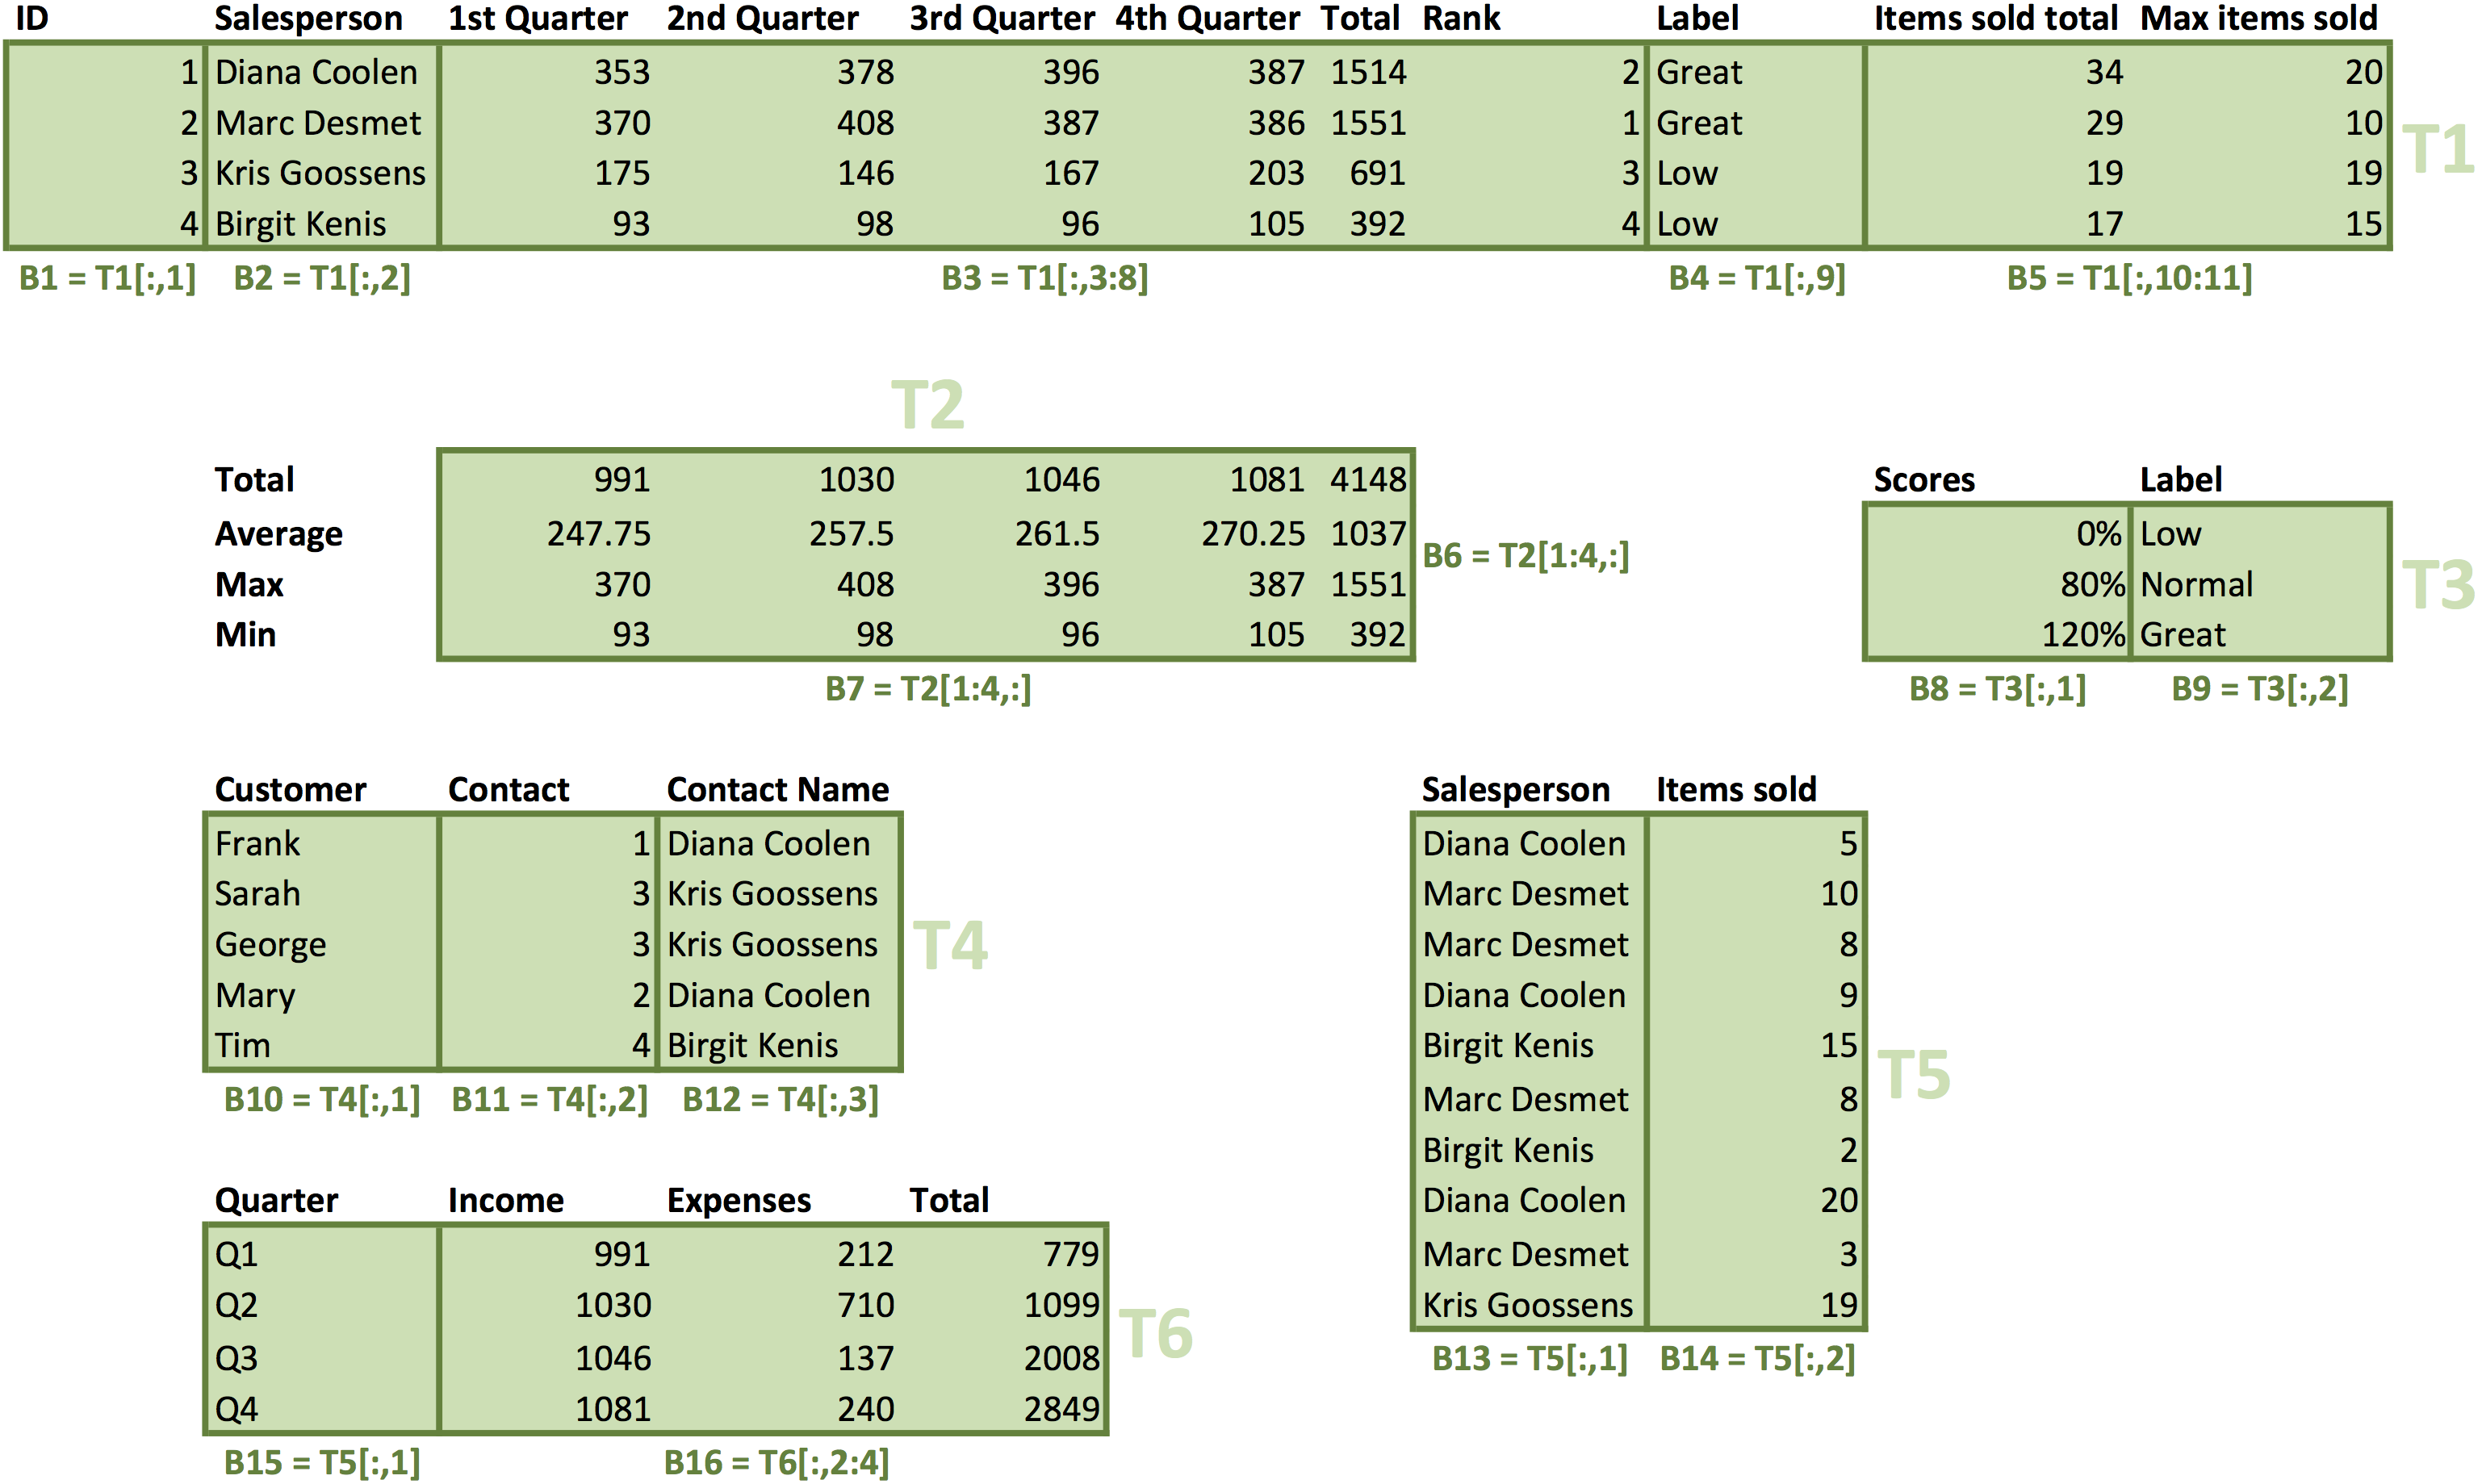
\includegraphics[width=1\textwidth]{figures/Demo2.png}
  \end{center}
  \vspace{-10pt}
  \caption{
    Example spreadsheet (black words and numbers only).
    Green background indicate headerless tables, dark borders indicate maximal type-consistent blocks.
    Most tables only contain type-consistent columns, however, table~$T_2$ also contains type-consistent row.
    This example was created by combining several Excel sheets from several exercise sessions.
    % I guess you want to save space by having everything in one figure, but it might be useful to have a smaller figure on the first page just to explain this example in a bit more detail (or use a smaller example here); it's quite overwhelming now}
  }
  \label{fig:main_example}
\end{subfigure}
\hfill
\begin{subfigure}{.35\textwidth}
  {\footnotesize
    \begin{align*}
      % Table 1
      &~\ecseries{\range{T_{1}}{\rangeall}{1}} \\
%
%      &~\ecperm{\range{T_{1}}{\rangeall}{1}}, \ecperm{\range{T_{1}}{\rangeall}{8}} \\
%
      &~\ecrank{\range{T_{1}}{\rangeall}{8}}{\range{T_{1}}{\rangeall}{7}}\\
      &~\ecrank{\range{T_{1}}{\rangeall}{8}}{\range{T_{1}}{\rangeall}{3}}^1, \ecrank{\range{T_{1}}{\rangeall}{8}}{\range{T_{1}}{\rangeall}{4}}^1 \\
      &~\ecrank{\range{T_{1}}{\rangeall}{1}}{\range{T_{1}}{\rangeall}{5}}^1 , \ecrank{\range{T_{1}}{\rangeall}{1}}{\range{T_{1}}{\rangeall}{6}}^1 \\
      &~\ecrank{\range{T_{1}}{\rangeall}{1}}{\range{T_{1}}{\rangeall}{10}}^1 \\
%
      &~\ecsumr{\range{T_{1}}{\rangeall}{7}}{\range{T_{1}}{\rangeall}{\rangeto{3}{6}}} \\
%
      &~\ecaggif{\textit{SUM}}{\range{T_{1}}{\rangeall}{10}}{\range{T_{5}}{\rangeall}{1}}{\range{T_{1}}{\rangeall}{2}}{\range{T_{5}}{\rangeall}{2}} \\
%
      &~\ecaggif{\textit{MAX}}{\range{T_{1}}{\rangeall}{11}}{\range{T_{5}}{\rangeall}{1}}{\range{T_{1}}{\rangeall}{2}}{\range{T_{5}}{\rangeall}{2}} \\
%
	  % Table 2
      &~\ecsumc{\range{T_{2}}{1}{\rangeall}}{\range{T_{1}}{\rangeall}{\rangeto{3}{7}}} \\
%
      &~\ecaggc{\textit{AVERAGE}}{\range{T_{2}}{2}{\rangeall}}{\range{T_{1}}{\rangeall}{\rangeto{3}{7}}} \\
%
      &~\ecaggc{\textit{MAX}}{\range{T_{2}}{3}{\rangeall}}{\range{T_{1}}{\rangeall}{\rangeto{3}{7}}},  \\
%
      &~\ecaggc{\textit{MIN}}{\range{T_{2}}{4}{\rangeall}}{\range{T_{1}}{\rangeall}{\rangeto{3}{7}}} \\
%
	  % Table 4
      &~\eclookup{\range{T_{4}}{\rangeall}{2}}{\range{T_{4}}{\rangeall}{3}}{\range{T_{1}}{\rangeall}{2}}{\range{T_{1}}{\rangeall}{1}}^2 \\
%
      &~\eclookup{\range{T_{4}}{\rangeall}{3}}{\range{T_{4}}{\rangeall}{2}}{\range{T_{1}}{\rangeall}{1}}{\range{T_{1}}{\rangeall}{2}} \\
%
	  % Table 6
      &~\ecsumc{\range{T_{6}}{\rangeall}{2}}{\range{T_{1}}{\rangeall}{\rangeto{3}{6}}} \\
%
      &~\range{T_{6}}{\rangeall}{4} = PREV(\range{T_{6}}{\rangeall}{4}) + \range{T_{6}}{\rangeall}{2} - \range{T_{6}}{\rangeall}{3}
    \end{align*}}
  \vspace{-10pt}
  \caption{Constraints present in the running example (left), except \textit{ALLDIFFERENT} (16), \textit{PERMUTATION} (2) and \textit{FOREIGNKEY} (5).
  $^1$(Spurious constraints) $^2$(Not present in original source)}
  \label{fig:sol_example}
\end{subfigure}
  \caption{Running example}
\end{figure*}


\section{Formalization}\label{sec:formalization}
Our goal is to automatically discover constraints (functions and relations) between the rows and the columns of tables in a spreadsheet. This is applicable not just to data from spreadsheets, but to any data in tabular form, hence the name.

%An example spreadsheet with tables is given in Figure~\ref{fig:main_example}, we will use this as running example throughout the paper.

We first introduce some terminology and the concept of a \template, after which we define the problem and make some additional considerations.

\subsection{Terminology}
Spreadsheets and tabular data may conceptually consist of multiple tables, such as in Figure~\ref{fig:main_example}. Note that a table can contain a header; however, we wish to reason over entire rows and columns of data, and hence we will consider \textbf{headerless tables} only.

Formally, a (headerless) table is an $n \times m$ matrix. Each entry is called a \textit{cell}.
A cell has a {\bf type}, which can be numeric or textual. We further distinguish numeric types in subtypes: integer and float. We also consider \textit{None} as a special type when a cell is empty; \textit{None} is a subtype of all other types.

A row or a column is \textbf{type-consistent} if all cells in that row or column are of the same base type, i.e. numeric or textual.
We will use notation $T[a,{:}]$ to refer to the $a$-th row of table $T$ and similarly $T[{:},a]$ for the $a$-th column.
For example, in Figure~\ref{fig:main_example}, $T_1[1,:] = [1,2,3,4]$ and $T_5[:,1] = ['$Diana Coolen$', 5]$.
$T_5[:,1]$ is not type-consistent while $T_1[1,:]$ is.
%We will write \textbf{vector} to refer to a single row or column when its orientation does not matter.

The most important concept is that of a \textbf{block}. 
\begin{definition}
A \textbf{block} has to satisfy three conditions: 1) it contains only entire rows or entire columns of a single headerless table 2) it is contiguous and 3) it is type-consistent.
The rows or columns have to be contiguous in the original table meaning that they must visually form a block in the table; and each of the rows/columns has to be of the same type. 
If it contains only rows we say it has \textit{row-orientation}, if only columns, \textit{column-orientation}. 
\end{definition}

In line with this definition, we can use the following notation to refer to blocks: $B = T[\rangeto{a}{b},:]$ for a row-oriented block containing rows $a$ to $b$ in table $T$; and similarly $B = T[{:},\rangeto{a}{b}]$ for a column-oriented block.
We will refer to the \textit{vectors} of a block when we wish to refer to its rows/columns independently of their orientation.


A block has the following properties:
\begin{itemize}
\item \textit{type}: a block is type-consistent, so it has a type
\item \textit{table}: the table that the block belongs to
\item \textit{orientation}: either row-oriented or column-oriented
\item \textit{size}: the number of vectors a block contains
\item \textit{length}: the length of its vectors; as all vectors are from the same table, they always have the same length.
\item \textit{rows}: the number of rows in the block
(in row-oriented blocks this is equivalent to the size)
\item \textit{columns}: the number of columns in the block (in row-oriented blocks this is equivalent to the length)
\end{itemize}

%We call a group $G$ \textit{numeric} (\textit{textual}, etc), written as \textit{numeric(G)}, if all its vectors contain numeric (textual, etc) elements.

%For notational convenience, we will refer to vectors in {\rm roman} and to groups in {\bf bold}. {\bf CHECK}

\begin{example}
Consider the (headerless) table~$T_1$ in Figure~\ref{fig:main_example}.
Its rows are not type consistent (i.e. they contain both numeric and textual data).
However, the table can be partitioned into five column-oriented blocks $B_1, B_2, B_3, B_4, B_5$, as shown in the figure ($B_1 = \range{T_1}{\rangeall}{1}$, $B_2 = \range{T_1}{\rangeall}{2}$, $B_3 = \range{T_1}{\rangeall}{\rangeto{3}{8}}$, \dots).
% {\small
% B_1 = \range{T_1}{\rangeall}{1},
% B_2 = \range{T_1}{\rangeall}{2},
% B_3 = \range{T_1}{\rangeall}{\rangeto{3}{8}},
% B_4 = \range{T_1}{\rangeall}{9},
% B_5 = \range{T_1}{\rangeall}{\rangeto{10}{11}}
\end{example}

\begin{definition}
\textbf{Block containment $\sqsubseteq$.} 
A block $B'$ is contained in a block $B$, $B' \sqsubseteq B$, iff both are valid blocks (contiguous, type consistent) with the same orientation and table, and each of the vectors in $B'$ is also in $B$. For row-oriented blocks: $B' \sqsubseteq B \Leftrightarrow B=\range{T}{\rangeto{a}{b}}{\rangeall} \wedge B'=\range{T}{\rangeto{a'}{b'}}{\rangeall} \wedge a \leq a' \wedge b' \leq b$ and similarly for column-oriented blocks.
\end{definition}

We will sometimes write that $B'$ is a \textit{subblock} of $B$ or that $B$ is a \textit{superblock} of $B'$.
%
An example of block containment is $T_1[:,\rangeto{3}{6}] \sqsubseteq T_1[:,\rangeto{3}{8}] $, which contains the sales numbers of all employees for the four quarters.


\begin{table*}[!h]
\caption{
  Overview of constraint templates implemented in \sname.
  Templates marked with $\dagger$ are \textit{aggregate} templates, the table shows the version for sum but \sname also supports max, min, average, product and count.
  Subgroups in normal font have to be vectors, whereas subgroups in \textbf{bold} may contain more than one vector.
  Templates marked with $*$ are \textit{structural}, i.e. they are not functional and cannot be implemented in most spreadsheet software.
  $\discrete(x)$ is a shortcut for: $\textual(x) \lor \numeric(x)$.
  {\small\luc{maybe say s.th. about some fancy constraints: example of a more complex one in the text (what does conditional mean, aggregate ... )}}
}
\label{table:constraints}
  {\centering
  \begin{tabularx}{\textwidth}{l X X}
    \textbf{\CName} & \textbf{\CSignature} & \textbf{\CFunction}\\ \hline \hline
    $\ecalldiff{\sg_x}^*$
      & $\discrete(\sg_x)$
      
      & All values in $\sg_x$ are different. $i \neq j$: $\sg_x[i] \neq \sg_x[j]$
      \\[\PADSEP] \hline

    $\ecperm{\sg_x}^*$
      & $\numeric(\sg_{x})$, $\ecalldiff{\sg_{x}}$
      
      & The values in $\sg_{x}$ are a permutation of the numbers $1$ through $\plength(\sg_{x})$.
      \\ \hline

    \ecseries{\sg_x}
      & $\integer(\sg_{x})$ and $\ecperm{\sg_{x}}$
      
      & $\sg_{x}[1] = 1$ and $\sg_{x}[i] = \sg_{x}[i - 1] + 1$.
      \\[\PADSEP] \hline

    $\ecfkey{\sg_{fk}}{\sg_{pk}}^*$
      & $\sg_{\mathit{fk}}$ and~$\sg_{pk}$ are $\discrete$; they must have different $\ptable$s but the same $\ptype$; and $\ecalldiff{\sbl{pk}}$

      & Every value in~$\sg_{fk}$ also exist in~$\sg_{pk}$ \\[\PADSEP] \hline

    \eclookup{\sbl{r}}{\sbl{fk}}{\sbl{pk}}{\sbl{val}}
      & $\sbl{fk}$ and $\sbl{pk}$ are $\discrete$; arguments $\{\sbl{fk}, \sbl{r}\}$ and $\{\sbl{pk}, \sbl{val}\}$ within the same set have the same \plength, \ptable and \por; $\sbl{r}$ and~$\sbl{val}$ have the same type; and \ecfkey{\sbl{fk}}{\sbl{pk}}.
      
      & $\sbl{r}[i] = \sbl{val}[j]$ where $\sbl{pk}[j] = \sbl{fk}[i]$
      \\[\PADSEP] \hline

    \eclookupfuzzy{\sbl{r}}{\sbl{fk}}{\sbl{pk}}{\sbl{val}}
      & \textit{Same as lookup}
      
      & $\sbl{r}[i] = \sbl{val}[j]$ where $\sbl{pk}[j] \leq \sbl{fk}[i]$, $j$~maximal
      \\[\PADSEP] \hline

    \eclookupprod{\sbl{r}}{\sbl{1}}{\sbl{fk}}{\sbl{pk}}{\sbl{val}}
      & Arguments $\{\sg_{r}, \sg_{1}, \sg_{fk}\}$ are $\numeric$, arguments $\{\sg_{pk}, \sg_{val}\}$ are $\discrete$ and within both sets all arguments have the same \plength, \ptable and \por; also \ecfkey{\sg_{fk}}{\sg_{pk}}.
      
      & $\sbl{r}[i] = \sbl{1}[i] \times \eclookupf{\sbl{fk}}{\sbl{pk}}{\sbl{val}}{}[i]$.
      \\[\PADSEP] \hline

    \ecprod{\sg_r}{\sg_1}{\sg_2}
      & Arguments $\{\sg_{r}, \sg_{1}, \sg_{2}\}$ are all $\numeric$ and have the same $\plength$
      
      & $\sg_{r}[i] = \sg_{1}[i] \times \sg_{2}[i]$.
      \\[\PADSEP] \hline

    \ecdiff{\sg_r}{\sg_1}{\sg_2}
      & Arguments $\{\sg_{r}, \sg_{1}, \sg_{2}\}$ are all $\numeric$ and have the same $\plength$ and $ \por$
      
      & $\sg_{r}[i] = \sg_{1}[i] - \sg_{2}[i]$.
      \\[\PADSEP] \hline

    \ecproj{\sg_r}{\mathbf{\sg_x}}
      & Arguments $\{\sg_{r}, \mathbf{\sg_x}\}$ all have the same $\plength$, $\por$, $\ptable$ and $\ptype$; $\mathbf{\sg_x}$ contains at least~2 vectors; and $\sg_r = \mathit{SUM}_{\por(\mathbf{\sg_x})}(\mathbf{\sg_x})$
      
      & At every position~$i$ in $1$ through $\plength(\sg_{r})$ there is exactly one vector~$v$ in $\mathbf{\sg_x}$ such that $v[i]$ is a non-blank value, then $v[i] = \sg_{r}[i]$.
      \\[\PADSEP] \hline

    \ecrank{\sg_r}{\sg_x}
      & $\integer(\sg_{r})$; $\numeric(\sg_{x})$; and $\plength(\sg_{r}) = \plength(\sg_{x})$
      
      & The values in $\sg_{r}$ represent the rank (from largest to smallest) of the values in $\sg_{x}$ (including ties)
      \\[\PADSEP] \hline

    \ectotal{\sg_r}{\sg_{pos}}{\sg_{neg}}
      & Arguments $\{\sg_{r}, \sg_{pos}, \sg_{neg}\}$ are all $\numeric$ and all have the same $\plength$, which is at least $2$
      
      & $\sg_{r}[i] = \sg_{r}[i - 1] + \sg_{pos}[i] - \sg_{neg}[i]$.
      \\[\PADSEP] \hline

    $\ecsumr{\sg_r}{\mathbf{\sg_x}}^\dagger$
      & $\sg_r$ and $\mathbf{\sg_x}$ are $\numeric$; $\pcols(\mathbf{\sg_x}) \geq 2$; and $\prows(\mathbf{\sg_x}) = \plength(\sg_r)$
      
      & $B_r[i] = \sum_{j = 1}^{\pcols(\bsbl{x})} \mathit{row}(i, \bsbl{x})[j]$
      \\[\PADSEP] \hline

    $\ecsumc{\sg_r}{\mathbf{\sg_x}}^\dagger$
      & $\sg_r$ and $\mathbf{\sg_x}$ are $\numeric$; $\prows(\mathbf{\sg_x}) \geq 2$; and $\pcols(\mathbf{\sg_x}) = \plength(\sg_r)$
      
      & $B_r[i] = \sum_{j = 1}^{\prows(\bsbl{x})} \mathit{column}(i, \bsbl{x})[j]$
      \\[\PADSEP] \hline

    $\ecsumif{\sg_r}{\sg_{fk}}{\sg_{pk}}{\sg_{val}}^\dagger$
      & $\sg_{fk}, \sg_{pk}$ are $\discrete$; $\sg_{r}, \sg_{val}$ are $\numeric$; within the sets $\{\sg_{val}, \sg_{fk}\}$ and $\{\sg_{pk}, \sg_{r}\}$ arguments have the same $\plength$ and $\por$; $\sg_{fk}$ and $\sg_{val}$ have the same $\ptable$; $\sg_{fk}$ and $\sg_{pk}$ must have different $\ptable$s but the same $\ptype$; and \ecalldiff{\sg_{pk}}
      
      & \[ B_r[i] = \sum_{j=1}^{\plength(B_{\textit{val}})} \begin{cases}
          \sg_{val}[j] & \text{if } \sg_{fk}[j] = \sg_{pk}[i] \\
          0 & \text{otherwise}
        \end{cases}
      \] \\[\PADSEP] \hline
      
    \ecsumprod{\sg_r}{\sg_1}{\sg_2}
      & Arguments $\{\sg_r, \sg_1, \sg_2\}$ are $\numeric$; $\plength(\sg_{1}) = \plength(\sg_{2}) \geq 2$; and $\prows(\sg_{r}) = \pcols(\sg_{r}) = 1$
      
      & $\sg_{r}[1] = \sum_{j = 1}^{\plength(\sg_{1})} \sg_{1}[j] \times \sg_{2}[j]$.
  \end{tabularx}}

\end{table*}

\newcommand{\sigc}{\ensuremath{\format{Sig}_s}}
\newcommand{\defc}{\ensuremath{\format{Def}_s}}

\subsection{Constraint templates}
The goal is to learn constraints over blocks in the data. The knowledge needed to learn a constraint is expressed through {\template}s.
%
A \template $s$ is a triple $t = \textit{(\CName, \CSignature, \CFunction)}$:
%Let us elaborate on this:
\begin{itemize}
\item
\textit{\CName}  specifies the syntactic form of the constraint $s(B_1, ...,B_n)$, that is, the name of the template together
with $n$ abstract arguments $B_i$.
Thus a constraint is viewed as a relation or predicate of arity $n$ in first order logic.
Note that a function $B_r=f(B_1,...,B_n)$ can be represented with the $(n{+}1)$-ary predicate $s_f(B_r,B_1,...,B_n)$.
Each argument will have to be instantiated with a block.
% the list of its variables $v_1,\dots,v_n$.  In ILP terminology, it is known as vocabulary.

\item \textit{\CSignature} defines the requirements that the arguments of the predicate must satisfy.
This can concern properties of individual blocks as well as relations between properties of arguments, for example that the corresponding blocks must belong to the same table or have equal length.
In terms of logical and relational learning \cite{luc_book}, the \CSignature is known as the {\em bias} of the learner, it specifies when the arguments of a constraint are well-formed.
We can capture this bias for a template~$s$ using a predicate $\sigc$.
\item \textit{\CFunction} is the actual definition of the constraint that specifies when the constraint holds.
Given an assignment of blocks to its arguments, it can be used to verify whether the constraint is satisfied or not by the actual data present in the blocks. %holds, in practice this will be a function that can be called when
%the arguments are full instantiated to decide whether the constraint is satisfied or not.
In logical and relational learning this is known as the background knowledge.
We introduce the predicate \defc~to capture this background knowledge for a template~$s$.
\end{itemize}

\begin{example}
The constraint templates implemented in \sname are defined in Table~\ref{table:constraints}.
A non-trivial example is, for example, the constraint template for the row-based sum:

\begin{itemize}
  \item \CName: $\ecsumr{\sg_r}{\mathbf{\sg_x}}$, for arguments $\sg_r$ and $\mathbf{\sg_x}$.
  
  \item \CSignature: $\sg_r$ has to be a single vector ($\textit{size}=1$) while $\mathbf{\sg_x}$ can be a block ($\textit{size}>=1$), which can be derived from the use of a normal or \textbf{bold} font.
  Both blocks have to be numeric.
  This constraint is orientation-specific, so it requires that the number of rows in $\mathbf{\sg_x}$ equals the length of $\sg_r$.
  Moreover, we add to the bias that the number of columns to sum over is at least~$2$.
  
  \item \CFunction: each value in the vector $\sg_{r}$ is obtained by summing over the corresponding row in $\mathbf{\sg_x}$.
  For example, $B_r = [12, 7]$ and $\mathbf{\sg_x}$ consists of columns: $[5, 15]$, $[7, -8]$.
\end{itemize}
\end{example}


It is helpful to see the analogy of constraint templates with first order logic (FOL) and constraint satisfaction.
From a FOL perspective, a constraint of the form $\ecrank{B_r}{B_x}$ can be seen as a predicate $\textit{RANK}(B_r, B_x)$ where \textit{RANK} is the name of the predicate and its arguments~$B_r$ and~$B_x$ are terms, which can be seen as either uninstantiated variables or as concrete values.
This also holds in our setting, where an instantiation of a variable corresponds to a concrete block.
For example, for the spreadsheet in Figure~\ref{fig:main_example}, when we write $\ecrank{\range{T_1}{\rangeall}{8}}{\range{T_1}{\rangeall}{7}}$, then the value of $B_r$ is the $8$th vector in $T_1$: $B_r = \range{T_1}{\rangeall}{8} = [2,1,3,4]$ and the value of $B_x$ is the $7$th vector: $B_x = \range{T_1}{\rangeall}{7} = [1514, 1551, 691, 392]$.

%When looking into constraints like \textit{$B$ = RANK($A$)}, it is helpful to see the analogy with both first order logic (FOL) and with constraint satisfaction problems.
%From a FOL perspective, the name of the constraint ($\mathit{RANK}$) is just the predicate, and the arguments $B$ and $A$ are the terms, which can be seen as either uninstantiated variables or as values (concrete groups with values).
%This also holds in our setting: when we write
%      $\ecrank{\range{T}{\rangeall}{8}}{\range{T}{\rangeall}{7}}$,
%we can interpret the argument ${\range{T}{\rangeall}{8}}$ as a group variable that would apply to any table $T$ (provided~$T$ has an 8th column).
%So, $T$ is viewed as table variable here, with the effect that  ${\range{T}{\rangeall}{8}}$ is a group variable.

With this interpretation, we can speak about the signature and definition of a constraint template being \textit{satisfied}.
We say that a signature (definition) of a constraint template~$s$ with $n$ arguments is satisfied by the blocks $(B_1, ..., B_n)$ if $\sigc(B_1, ..., B_n)$ (respectively $\defc(B_1, ..., B_n)$) is satisfied.
Likewise, the template is satisfied if both the signature and definition are satisfied; in logic programming and logical relational learning, we would define the predicate~$s$ using a Prolog like clause: $s(B_1, ..., B_n) \leftarrow \sigc(B_1, ..., B_n) \wedge \defc(B_1, ..., B_n)$.
Under this interpretation, the term constraint and constraint template can be used interchangeably.

\begin{definition}
A \textbf{valid argument assignment} of a constraint $s$ is a tuple of blocks $(B_1, ..., B_n)$ such that $s(B_1, ..., B_n)$ is satisfied, that is, both the signature and the definition of the corresponding constraint template are satisfied by the assignment of $(B_1, ..., B_n)$ to the arguments.
\end{definition}





\subsection{Problem Definition}\label{sec:problem_statement}
The problem of learning constraints from tabular data can be seen as an inverse {\em constraint satisfaction problem} (CSP).
In a CSP one is given a set of constraints over variables that must all be satisfied, and the goal is to find an instantiation of all the variables that satisfies these constraints.
In the context of spreadsheets, the variables would be (blocks of) cells, and one would be given the actual constraints and functions with the goal of finding the values in the cells.
The inverse problem is, given only an instantiation of the cells, to find the constraints that are satisfied in the spreadsheet.

We define the inverse problem, that is the {\bf Tabular Constraint Learning Problem}, as follows:
%
\begin{definition} \textit{Tabular Constraint Learning.}\label{def:problem_statement}\\
{\bf Given} a set of instantiated blocks~${\cal B}$ over tables~${\cal T}$ and a set of {\template}s ${\cal S}$: {\bf find} all constraints $s(B'_1, ..., B'_n)$ where $s \in {\cal S}$, $\forall i: B_i' \sqsubseteq B_i \in {\cal B}$ and $(B'_1, ..., B'_n)$ is a satisfied argument assignment of the template~$s$.
\end{definition}
% Let us now define what it means for a constraint from \template to hold in general. Let $t$ be a \template, $S$ be a mapping from variables to the subgroups of \groups, and $C$ be the constraint $t^S$, then $C$ \textit{holds} iff all constraints in $\text{\CSignature}^S$ and $\text{\CFunction}^S$ of $C$ hold.
% \sergey{moved from formalization END}

%Here we formalize the statement in terms of \template and group assignments as follows:
%   \begin{tabular}{ll}
%     \multicolumn{2}{l}{{\textbf{Tabular Constraint Learning Problem}}}\\
%     \textbf{Given:}& the set of all groups $\groups$ and of \template $\constraints$\\
%     \textbf{Find:}&  all constraints $C$ over \groups for each template $t$ in \constraints \\
%   \end{tabular}

Blocks and tables are expected to be given, in Section~\ref{sec:approach} we will discuss how these can be extracted from a spreadsheet.
Figure~\ref{fig:sol_example} shows the solution to the tabular constraint learning problem when applied on the blocks of Figure~\ref{fig:main_example} and constraint templates listed in Table~\ref{table:constraints}.

\subsection{Other considerations}

\subsubsection{Dependencies}
\label{sec:form:dependencies}
In Table~\ref{table:constraints} one can see that for some constraints we used the predicate of another constraint in its signature, e.g. for \textit{PERMUTATION}. This expresses a dependency of the constraint on that other constraint. This can be interpreted as follows: the signature of the constraint consists of its own signature plus the signature of the depending constraint, and its definition of its own definition plus the definition of the depending constraint.
In FOL, we can see that one constraint entails the other, for example if $\ecperm{\sg_x}$ holds for a block $\sg_x$, then $\ecalldiff{\sg_{x}}$ also holds.

Apart from easing the specification of the signature and definition, in Section~\ref{sec:approach} we will see how such dependencies can be used to speed up the search for constraints.

\subsubsection{Redundancies}
\label{sec:form:redundancies}
Depending on the application, some constraints in the solution to the tabular constraint learning problem may be considered \textit{redundant}. This is because constraints may be logically equivalent or may be implied by other constraints, e.g. if you know $\ecperm{B_x}$, $\ecalldiff{B_x}$ is redundant.

Within the same constraint, there can be equivalent argument assignments if the order of some of the arguments does not matter. For example for the product constraint, $\ecprod{\sg_r}{\sg_1}{\sg_2} \equiv \ecprod{\sg_r}{\sg_2}{\sg_1}$ so one can be considered redundant to the other.

Two different constraints may be logically equivalent due to their nature, e.g. for addition/subtraction and product/division: $\ecprod{\sg_r}{\sg_1}{\sg_2} \equiv \ecdiv{\sg_1}{\sg_r}{\sg_2}$.

When the data has rows or columns containing exactly the same data, then any constraint with such a vector in its argument assignment will also have an argument assignment with the other equivalent vectors.

Dealing with redundancy is often application-dependent.
Therefore, in Section~\ref{sec:approach} we will first explain our generic method for finding all constraints, before describing some optimizations that avoid obvious equivalences (Section~\ref{sec:opts}).
Later, we will investigate the impact of redundancy in the experiments.

%More formally, a constraint $c_1(G_1, ... G_n)$ \textit{implies} another constraint~$c_2(G'_1, ..., G'_m)$ whenever
%the  following statement holds: $$\forall G_i, G'_j : c_1(G_1, ... G_n) \rightarrow c_2(G'_1, ... G'_m).$$
%
%We shall only consider {\em range-restricted} implications, that is, we shall require that $\{G'_1, ..., G'_m\} \subseteq \{G_1, ..., G_n\}$.
%To simplify notation, and in line with logic programming, we shall often make the quantification implicit and simply write this as rules $ c_1(G_1, ... G_n) \rightarrow c_2(G'_1, ... G'_m)$.  We say that the first constraint is more specific than the second, and the second is more general.
%
%
%% where the second one ranges over a subsets of the arguments of the first, iff whenever the first constraint is true, the second must also be true. More formally, $\forall G'_1, ..., G'_n$ s.t. $\{G''_1, ..., G''_m\} \subseteq \{G'_1, ..., G'_n\},\, c_1(G'_1, ... G'_n) \rightarrow c_2(G''_1, ..., G''_m)$ll.
%
%\paragraph{Example}
%Consider the following implication:
%$$\ecperm{G} \rightarrow \ecalldiff{G}$$
%(it can be seen in Table~\ref{table:constraints} that both constraints only hold if $G$ is a vector).
%In this case the arguments are identical in both constraints.
%Given that the problem is to find the set of {\em all} constraints, and that the more general constraint is entailed
%by the more specific one, the $\ecdiff{G}$ constraint will be {\em redundant}.
%So, for most applications, it will be sufficient to output only the most specific one.
%
%A more involved example is
%$$\eclookup{G'_2}{G'_1}{H'_1}{H'_2} \rightarrow \ecfkey{G'_1}{H'_1}$$
%which states
%that a look-up constraint implies a foreign-key constraint. In the look-up constraint $\eclookup{G'_2}{G'_1}{H'_1}{H'_2}$ the values in the vector $G'_2$ are determined by looking up the corresponding value in vector $G'_1$ in vector $H'_1$ and returning the corresponding value in vector $H'_2$. In Figure~\ref{fig:main_example} we have $\eclookup{\range{T_{4}}{\rangeall}{3}}{\range{T_{4}}{\rangeall}{2}}{\range{T_{1}}{\rangeall}{1}}{\range{T_{1}}{\rangeall}{2}}$. This implies a foreign-key constraint $\ecfkey{G'_1}{H'_1}$ where each of the values in vector $G'_1$ must appear in $H'_1$ for the look-up to work.


%\tias{I am not defining a new problem for 'most specific canonical tabular constraint learning' because we loosely showed how implications and equivalences would be expressed, but not how to express canonicity and we did not claim that most specific is always best.}
%\tias{Note also that our method finds ALL constraints; it uses specificity to faster traverse the search space, but the resulting set of constraints found would be the same, whether or not using the specificity (see 4.2.1).}

%Let us introduce the version of tabular constraint learning by modifying Definition \ref{def:problem_statement} that takes into account the specificity relation between constraint templates.
%
%\begin{definition} \textit{Condensed Tabular Constraint Learning}\label{def:condensed_problem_statement}\\
%  Given a set of instantiated tables~${\cal T}$ (all cells have values), a set of {\template}s~${\cal S}$, a set of groups~${\cal G}$ over the tables~${\cal T}$, and the set of all specifity rules~\dependencies: find the set of all constraints $s(G_1', ..., G_n')$ that are satisfied  in ${\cal T}$, for which all $G_i' \subseteq G_i \in {\cal G}$, the (sub)groups $G_1', ... , G_n'$ satisfy the signature of the constraint template~$s \in {\cal C}$ and there is no $s'$ in ${\cal C}$ such that $s'(G_h',\dots,G_k')$ holds (for $1 \leq h \leq k \leq n$) and  $s'$ is more specific than $s$ in \dependencies.
%\end{definition}

% \begin{minipage}[c]{14em}
%   \vspace{5pt}
%   \begin{tabular}{ll}
%     \multicolumn{2}{l}{{\textbf{Condensed Tabular Constraint Learning Problem}}}\\
%     \vspace{-4pt}
%     &\\
%     \textbf{Given:}& the set of all groups $\groups$ and of \template's $\constraints$,\\
%     & a constraint specificity DAG \dependencies \\
%     \textbf{Find:}& all the most specific wrt \dependencies constraints $C$ over \groups\\
%     & for each $t$ in \constraints \\
%   \end{tabular}
%   \vspace{6pt}
% \end{minipage}

%This version explicitly takes into account the specificity of the constraints and invalidates some of the solutions that are entailed by the tabular other solutions.





\newcommand{\tcl}{Tabular Constraint Learning}
%\newcommand{\ctl}{Condensed Tabular Constraint Learning}
\section{Approach to Tabular Constraint Learning}\label{sec:approach}
The aim of our method is to detect constraints between rows and columns of tabular data. Recall that a valid argument assignment for a constraint is an assignment of a block to each of the arguments of the constraint, such that the signature and definition of the constraint template is satisfied.

Our proposed methodology contains the following steps:
\begin{enumerate}
\item Extract headerless tables from tabular data
\item Partition the tables into contiguous, type-consistent \textit{superblocks}
\item Generate for each constraint template all valid argument assignments in two steps:
\begin{enumerate}
\item For each constraint template~$s$, generate all assignments $(B_1, \ldots ,B_n)$ where each $B_i$ is a superblock and the $B_i$ are \textit{compatible} (defined below) with the signature of~$s$. 
\item For each generated assignment $(B_1, \ldots ,B_n)$ in 3a), find all valid constraints $s(B'_1, \ldots, B'_n)$ such that for all $i$ holds $B'_i \sqsubseteq B_i$ and the signature and definition of~$s$ are satisfied.
\end{enumerate}
\end{enumerate}

The core of our method is step 3. In principle, one could use a generate-and-test approach by generating all possible blocks from the superblock and testing each combination of blocks for each of the arguments of the constraints. However, each superblock of size $m$ has $m*(m+1)/2$ contiguous subblocks, meaning that a constraint with $n$ arguments would have to check $O(n^{m^2})$ combinations of blocks.

Instead, we divide this step into two parts: in step 3a, we will not reason over individual (sub)blocks and their data, but rather over the properties of the superblocks.
% and what combination of superblocks may lead to a valid argument assignment.\\
Consider table~$T_1$ in Figure~\ref{fig:main_example} and the $\mathit{SUM}_{row}$ constraint template.
Instead of considering all possible subblocks of $T_1$, we first reason over the properties of the superblocks.
For example, $B_2$ and $B_4$ are not numeric so they can be immediately discarded.
Superblocks~$B_1, B_3$ and $B_5$ are valid candidates for $B_r$, however, since they all have length~4, $\mathbf{B_x}$ needs at least 4~columns which is only satisfied by $B_3$.
So the assignments generated in step 3a would be $(B_1, B_3), (B_3, B_3), (B_5, B_3)$.

In step 3b, we start from an assignment $(B_1, \ldots, B_n)$ with superblocks $B_i$, and generate and test all possible (sub)block assignments to arguments using the properties and actual data of the blocks. As we only have to consider the blocks $B'_i \sqsubseteq B_i$ contained in each superblock, this is typically much easier. For the above example, each of the vectors of $B_6$ will be considered as candidate for the left-hand side, and one can enumerate all subblocks for the right-hand side and verify the signature (e.g. at least size $4$) and test whether for each row the definition is satisfied. %In practice, this can be optimized further.

We now describe in more detail how headerless tables are extracted (step 1, Section~\ref{sec:table_extraction}) and how superblocks are generated from them (step 2, Section~\ref{sec:make_groups}), how the candidate superblock assignments are generated (step 3a, Section~\ref{sec:algo:super}) and how the actual assignments are extracted from that (step 3b, Section~\ref{sec:algo:subgr}).
In Section~\ref{sec:opts} we describe a number of optimizations designed to speed up steps the algorithm.





\subsection{Table extraction}
\label{sec:table_extraction}
Many spreadsheets contain headers that provide hints at where the table(s) in the sheet are and what the meaning of the rows and columns is. However, detecting tables and headers is a complex problem on its own~\cite{header}. Furthermore, headers may be missing and their use often requires incorporating language-specific vocabulary, e.g. English.

\begin{figure}[t]
  \centering
  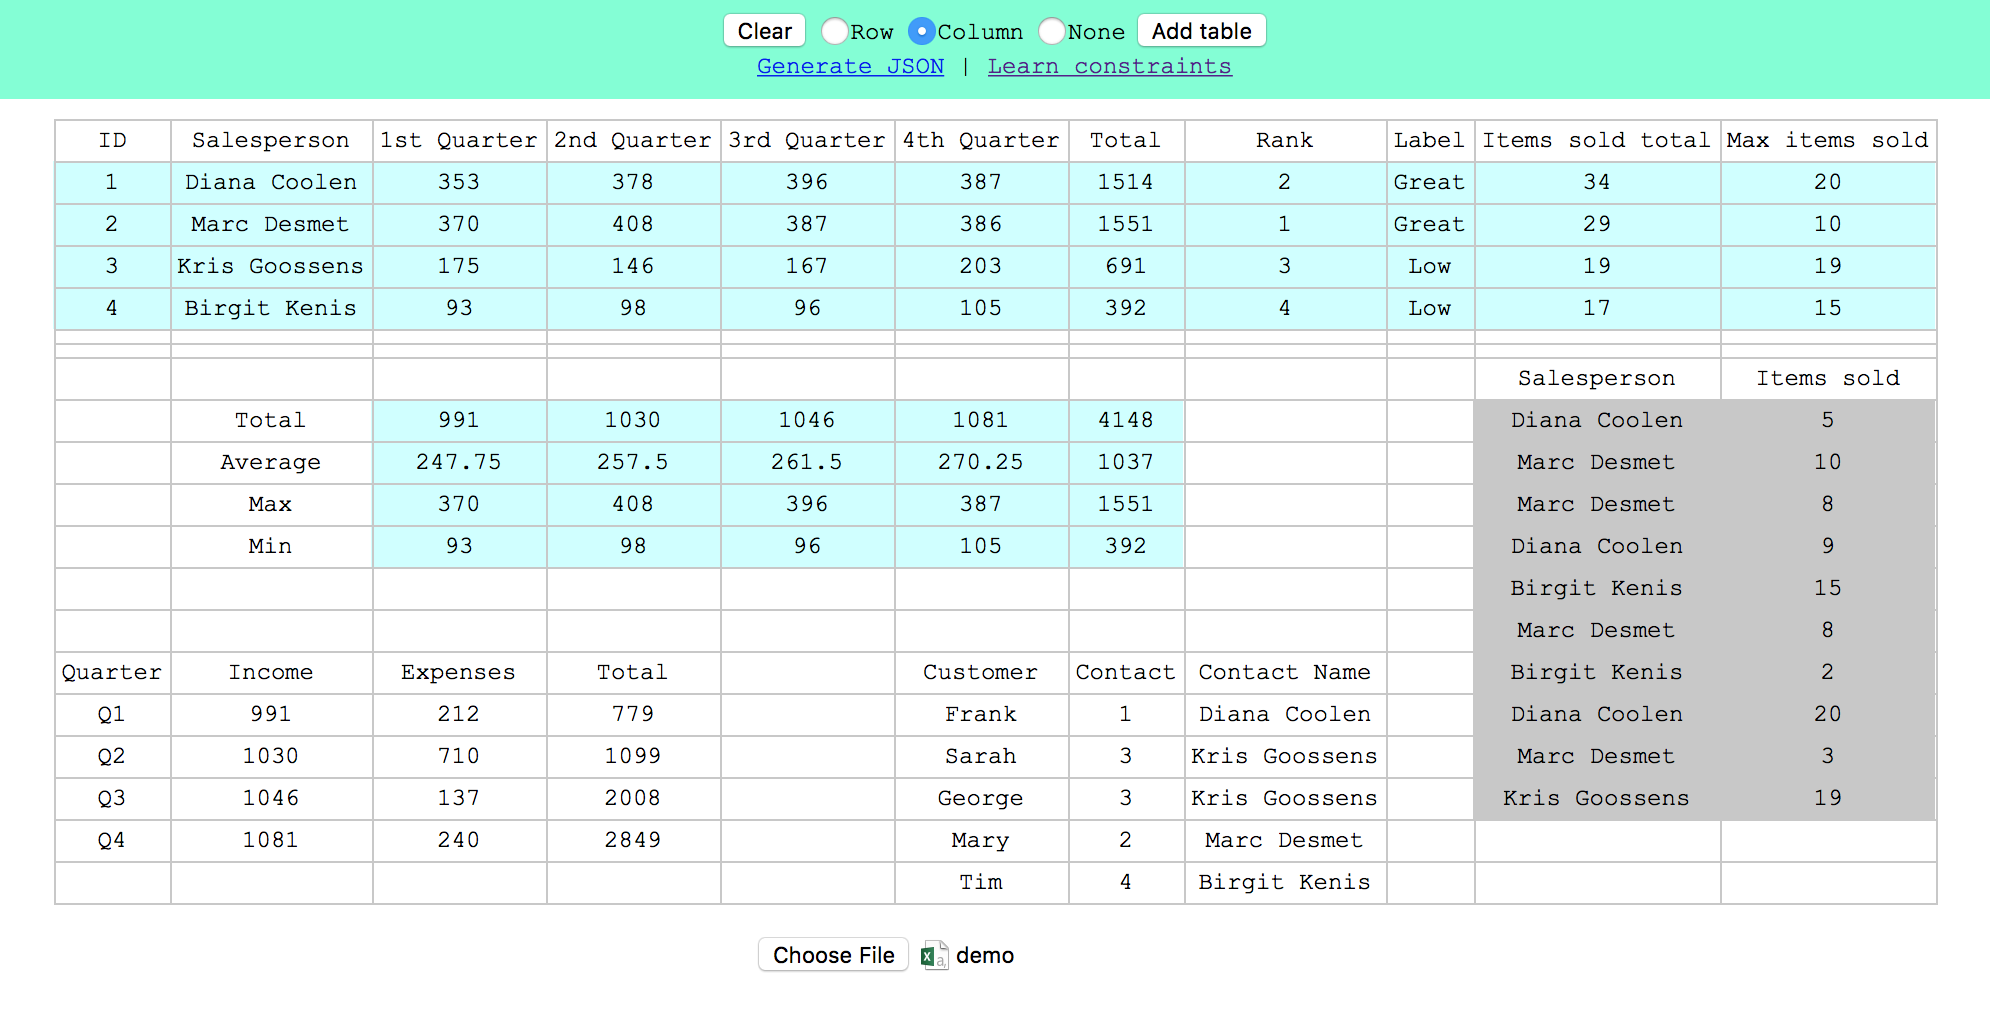
\includegraphics[width=1\linewidth]{figures/tabletool.png}
  \caption{This simple table selection tool allows users to select rectangular ranges of cells corresponding (headerless) tables, an explicit orientation can also be provided.}
  \label{fig:visual_tool}
\end{figure}

Instead, we assume tables are specified by means of their coordinates within a spreadsheet and optionally a fixed orientation of each table. The orientation can be used to indicate that a table should be interpreted as having only rows or only columns.

We developed two simple prototypes to help with the specification of the tables:
%This information can be provided manually or generated automatically.


\paragraph{Automatic detection}
%As mentioned above, automatic detection of headers and tables is a complex task.
%Therefore, we define a restricted setting in which the task becomes easy enough to be automated.
Under the following two assumptions, the table detection task becomes easy enough to be automated; 1) tables are rectangular blocks of data not containing any empty cells; and 2) tables are separated by at least one empty cell from other tables.
The sheet is then processed row by row, splitting each row into ranges of non-empty cells and appending them to adjacent ranges in the previous row.
Headers can be detected, for example, by checking if the first row or column contains only textual values. If a header row (column) is detected, it is removed from the table and the orientation of the table is fixed to columns (rows), otherwise, we assume there is no header and the orientation is not fixed.

\paragraph{Visual}
The above assumptions do not hold for many tables. However, since the specification of tables is usually easy for humans, we propose a second approach which allows users to indicate tables using a visual tool (Figure~\ref{fig:visual_tool}).
Users select tables excluding the header and optionally specify an orientation.
The tool then generates the specification of the tables automatically.





\subsection{Block detection} \label{sec:make_groups}
%A spreadsheet may contain multiple tables, and a table in turn will contain multiple (type-consistent) blocks.
The goal of the block detection step is to partition tables into maximally type-consistent (all-numeric or all-textual) blocks.
%We generate blocks automatically, partitioning tables into maximal type-consistent blocks.
First, we preprocess the spreadsheet data so that currency values and percentual values are transformed into their corresponding numeric (i.e. integer or floating point) representation (e.g. $2.75 \$$ as $2.75$ or $85\%$ as~$0.85$).
Then, each table is partitioned into maximal type-consistent blocks.

To find row-blocks, each row is treated as a vector and must be type-consistent; similarly for column-blocks. Then, adjacent vectors that are of the same type are merged to obtain the maximally type-consistent superblocks.


\subsection{Algorithm}
\label{sec:algo}
Our method assumes that constraint templates and maximal blocks are given and solves the \tcl~problem by checking for each template $s$: what combination of maximal blocks can satisfy the signature (\textit{superblock assignment}) and which specific \textit{subblock assignments} satisfy both the signature and the definition.
The pseudo-code of this approach is shown in Algorithm~\ref{algo:tcl}.
%For every constraint template~$s$, the algorithm first generates all combinations of superblocks (i.e. superblock assignments) that are consistent with the signature.
%In a second step it looks at every superblock assignment and finds subassignments that satisfy the signature and definition of~$s$.


This separation of checking the \textit{properties} of superblock assignments from checking the \textit{actual data} in the subblock assignment controls the exponential blow-up of combinations to test. Furthermore, we use constraint satisfaction technology in the first step to efficiently enumerate superblock assignments that are compatible with the signature. %These are the two key properties of our approach.

\newcommand{\temps}{\ensuremath{S}}
\begin{algorithm}[t]
  \begin{algorithmic}[1]
    \footnotesize
    \State \textbf{Input:} $\temps$ -- constraint templates, $\blocks$ -- maximal blocks
    \State \textbf{Output:} $C$ -- learned constraints

    \Procedure{LearnConstraints}{$\blocks$, $\temps$}
      \State $C \gets \emptyset$ %\Comment{The set of constraints}
      \ForAll{$s~\mathbf{in}~\temps$}
        %\State $n \gets$ number of arguments of template $s$
        \State $A \gets \generategroups(s, \blocks)$
        \ForAll{$(B_1, \dots, B_n) \in A$}
        \State $A' \gets \findassignment(s, (B_1,\dots,B_n))$
        \ForAll{$(B_1',\dots,B_n') \in A'$}
            \State $C \gets C \cup \{ c_s(B_1', \dots, B_n') \}$
          \EndFor
        \EndFor
      \EndFor
      \State \Return $C$
    \EndProcedure
\end{algorithmic}
\caption{Learn tabular constraints}
\label{algo:tcl}
\end{algorithm}





\subsubsection{Generating superblock assignments (Step 3a)}
\label{sec:algo:super}
\
% Let there be $b$ blocks and let~$s$ have~$n$ arguments, then a simple generate-and-test method would have to test $b^n$ combinations (given that blocks can be repeated), which can grow very rapidly with $b$, depending on $n$.

Given a constraint template~$s$ and the set of all maximal blocks~\blocks, the goal is to find all combinations of maximal blocks that are consistent with the constraint signature.
An argument assignment $(B_1, ... B_n)$ is \textit{consistent} with the signature of template $s$ if for each block $B_i$ there exists at least one subblock $B_i' \sqsubseteq B_i$ that satisfies the signature.

Furthermore, the choice of one argument can influence the possible candidates blocks for the other arguments, for example, if they must have the same length.
Instead of writing specialized code to generate and test the superblock assignments, we make use of the built-in reasoning mechanisms of constraint satisfaction solvers.

A Constraint Satisfaction Problem (CSP) is a triple $(V,D,C)$ where $V$ is a set of \textit{variables}, $D$ the domain of possible values each variable can take and $C$ the set of constraints over $V$ that must be satisfied.
In our case, we define one variable $V_i$ for each argument of a constraint template.
Each variable can be assigned each of the maximal blocks in \blocks, so the domain of the variables consists of $|\{\blocks\}|$ block identifiers.

%Finding candidate groups for a \template~$t$ can be seen as a Constraint Satisfaction Problem (CSP) dependent on the \CSignature of~$t$.
%For every argument in~$t$ we consider all groups~\groups (or all candidates from a more general constraint) and prune these candidate groups using their types and other requirements imposed by the templates \CSignature, such that a group~$G \in \groups$ is selected if there is at least one subgroup~$G' \subseteq G$ that satisfies the \CSignature.

To reason over the blocks, we add to the constraint program a set of background facts that contain the properties of each block, namely its type, table, orientation, size, length and number of rows and columns.
%The actual constraints correspond to the requirements defined in the signature, such as whether arguments are of a certain type, have certain dependencies or have to be equal length or orientation, etc.
%
% \tias{More detailed description of the properties commented out, feel free to put in}
%Translation:
%\begin{description}
%  \item[Type] Require group that has supertype (e.g. integer => require numeric group, because subgroup might be integer)
%  \item[Length] Require group to have exact length (subgroups have the same length)
%  \item[Vectors / columns / rows] Require group to have at least the amount of vectors, columns, rows required
%  \item[Dependency] Fix dependent variables, for every assignment construct CSP that attempts to find values for the other variables
%  \item[Same length / table / orientation] Require groups to gave the same length table ...
%\end{description}
%
\begin{table}[t]
  \caption{Translation of signature requirements to superblock constraints. The requirements that do not need to be relaxed are: $\plength(B) = x$, $\por(B) = x$, $\ptable(B) = x$ and $\psize(B) \geq x$.}
  \label{tbl:translation}
  \begin{tabularx}{\linewidth}{lX}
    \textbf{Requirement} & \textbf{Superblock constraint} \\ \hline \hline
    $\ptype(B) = x$ & $\mathit{basetype}(\ptype(B)) = \mathit{basetype}(x)$ \\ \hline
    $\psize(B) = x$ & $\psize(B) \geq x$ \\ \hline
    $\pcols(B) = x$ & $\mathit{if}~\por(B) = \mathit{column}: \pcols(B) \geq x$ \\ 
    & $\mathit{if}~\por(B) = \mathit{row}: \pcols(B) = x$ \\ \hline
    $\prows(B) = x$ & $\mathit{if}~\por(B) = \mathit{column}: \prows(B) = x$ \\ 
    & $\mathit{if}~\por(B) = \mathit{row}: \prows(B) \geq x$
  \end{tabularx}
\end{table}
%
The actual constraints must enforce that a superblock assignment is \textit{consistent} with the requirements defined in the signature.
%
%In order for our approach to be complete, the signature constraints can not always be enforced directly on a block.
%If a block matches the signature it is a valid candidate, however, if it does not there might exist subblocks that still satisfy the signature.
%\begin{example}
%  Consider, for example, the constraint template \ecseries{x} and a superblock candidate~$B$ for~$x$ containing both integer and floating point values.
%  While the signature of the template requires~$x$ to be integer we cannot discard~$B$ since there might be subblocks~$B' \sqsubseteq B$ that only contain integer values and satisfy the signature.
%\end{example}

Table~\ref{tbl:translation} shows how the conversion from requirements of the signature to CSP constraints works:
Requirements on the lengths, orientations and tables of blocks can be directly enforced since they are invariant under block containment($\sqsubseteq$).
Typing requirements need to be relaxed to check only for base types (numeric and textual).
Minimum sizes can be directly enforced, but exact size requirements are relaxed to minimum sizes, since blocks with two many vectors contain subblocks of the required size.
Finally, restrictions on the number of rows or columns behave as length or size constraints based on the orientation of the block they are applied to.
Subgroups of row-oriented (column-oriented) blocks will always have the same number of columns (rows), however, the number of rows (columns) might decrease.

The $\generategroups(\textit{s,\blocks})$ method will use these conversion rules to construct a CSP and query a solver for all solutions.
These solutions correspond to the valid superblock assignments for constraint template~$s$.

\begin{example}
%Br and Bx are numeric; rows(Bx) ⇤ 2; and columns(Bx ) = length(Br )

  Consider the constraint template $\ecsumc{\sg_r}{\mathbf{\sg_x}}$, then the generated CSP will contain two variables $V_r, V_x$ corresponding to arguments~$\sg_r$ and~$\mathbf{\sg_x}$.
  Given maximal blocks~\blocks, the domain of these variables are $D(V_r) = D(V_x) = \{ 1, \dots, |\blocks| \}$.
  Finally, the signature of $\ecsumc{\sg_r}{\mathbf{\sg_x}}$ (see Table~\ref{table:constraints}) will be translated into constraints:
  \begin{align*}
    & \numeric(V_r) \land \numeric(V_x) \land \prows(V_x) \geq 2 \\
    & (\por(V_x) = \mathit{row}) \Rightarrow (\pcols(V_x) \geq \plength(V_r)) \\
    & (\por(V_x) = \mathit{column}) \Rightarrow (\pcols(V_x) = \plength(V_r))
  \end{align*}
  %Every solution is a tuple of values for~$V_r$ and~$V_x$ corresponding directly with a superblock assignment over~\blocks.
\end{example}





\subsubsection{Generating subblock assignments (Step 3b)}
\label{sec:algo:subgr}
Given a superblock assignment $(B_1, \dots, B_n)$ from the previous step, the goal is to discover valid \textit{subassignments}, i.e. assignments of subblocks $(B'_1, \dots, B'_n)$ (for all $i$, $B'_i \subseteq B_i$) that satisfy both the signature and the definition of template~$s$.

%While the previous step reasoned about the \textit{properties} of blocks, in this step we will also reason about the actual \textit{content} of the blocks, that is, the data.
\begin{example}
  Consider the sum-over-rows constraint template $\ecsumr{\sg_r}{\mathbf{\sg_x}}$.
  An example superblock assignment from Figure~\ref{fig:main_example} is $(B_r, \mathbf{\sg_x}) = (\range{T_1}{\rangeall}{\rangeto{3}{8}}, \range{T_1}{\rangeall}{\rangeto{3}{8}})$.
  Note that this assignment does not satisfy the signature yet, $\sg_r$ contains more than one vector and $\psize(\mathbf{\sg_x}) \neq \plength(B_r)$.
  This step aims to generate subassignments $(B_r' \sqsubseteq B_r, \mathbf{B_x}' \sqsubseteq \mathbf{B_x})$ that \textit{do} satisfy the signature and test whether they satisfy the definition:
  $\forall i, \sbl{r}[i] = \sum_{j = 1}^{\pcols(\bsbl{x})} \mathit{row}(i, \bsbl{x})[j]$.
  In Figure~\ref{fig:main_example} there is exactly one such subassignment: $(\range{T_1}{\rangeall}{7}, \range{T_1}{\rangeall}{\rangeto{3}{6}})$.
\end{example}

In this step, we could also formulate the problem as a CSP. %However, the search space is much smaller, e.g. $O(nm^2)$ with $n$ the number of arguments of the template and $m$ the size of the largest block.
However, few CSP solvers support floating point numbers, which are prevalent in spreadsheets.
Furthermore, in a CSP approach we would have to \textit{ground} out the definition for each of the corresponding elements in the vectors.
This is inefficient, as already the blocks may not satisfy the signature or the first elements in the data may not satisfy the definition.

Hence, a simple generate-and-test will usually suffice.
%However, the actual implementation is specified for every constraint template separately, allowing different methods to be used based on the type of template.
%For this reason, the \sname system uses generate-and-test to implement $\findassignment$ for most constraint templates.
Given a superblock assignment, all disjoint subassignments are generated taking into account the required size, columns or rows.
For every (disjoint) subassignment the exact signature (e.g. subtypes will not have been checked yet) and definition will be tested and all satisfying subassignments are returned.

\begin{algorithm}[tbh]
  \begin{algorithmic}
    \footnotesize
    \Procedure{Subassignments}{$s$, $(B_1, \dots, B_n)$}
    \State $n \gets$ number of arguments of template $s$
    \State $A_{sub} \gets \emptyset$
    \ForAll{$(B_1', \dots, B_n') \textbf{ where } \forall i: B_i' \sqsubseteq B_i  \land \textit{disjoint}_{j \neq i}(B_i', B_j')$}
      \If{$\mathit{Sig}_s(B_1',\dots,B_n') \land \mathit{Def}_s(B_1',\dots,B_n')$}
        \State $A_{sub} \gets A_{sub} \cup \{ (B_1', \dots, B_n') \}$
      \EndIf
    \EndFor
\Return $A_{sub}$
\EndProcedure
\end{algorithmic}
\caption{Generate-and-test for $\findassignment$}
\label{algo:gen-test-subblocks}
\end{algorithm}




% \begin{verbatim}
% VERY PSEUDOcode:
% something recursive that handles vectors/
% subgroups differently like this?
% check(Groups, X, Test):
%   if |Groups| == 0:
%     forall i in ?: vector elements...
%       if not Test(X):
%         return []
%     return X
%   // else
%   all = []
%   Group = Groups.pop(0)
%   if vector(Group):
%     forall Vec in Group:
%       all += check(Groups, X + Vec, Test)
%   else:
%     forall Subgroup in Group:
%       all += check(Groups, X + Subgroup, Test)
%   return all
% \end{verbatim}

 %$G_1 = +(G_2, G_3) \leftrightarrow G_1 = +(G_3, G_2)$. \samuel{\tias{How are they stopped in the code? should be part of the pseud-code because not part of $Test(X)$?} will make it part of pseudo-code}

% \paragraph{Example 2, not used (should be replaced by pseudo-code above?)}
% Sum Product

% Implementation: finds subgroups based on assignments\\
% Method $Test(G_R, G_{O_1}, G_{O_2})$\\
% $If \lnot G_{O_1} < G_{O_2}: Reject~\#~Canonicity$\tias{ill-defined, $G_{O_1}$ is a group and $<$ not defined on it (on vector identifiers rather than content?)}\\
% $If data(G_R) = data(G_{O_1}) \bullet data(G_{O_2}): Accept$ \tias{does not show that reasons over content of vectors}
% \\\\
% Method $FindSubgroups(Assignments)$\\
% $Return \{ (G_R', G_{O_1}', G_{O_2}') | \exists (G_R, G_{O_1}, G_{O_2}) \in Assignments \land G_R' \subseteq G_R \land G_{O_1}' \subseteq G_{O_1} \land G_{O_2}' \subseteq G_{O_2} \land Test(G_R', G_{O_1}', G_{O_2}') \}$ \tias{does not enforce size of subgroups (e.g. vectors)?}





\subsection{Optimizations} \label{sec:opts}
This section discusses various design decisions and optimizations aimed at improving the speed and extensibility of our system as well as to eliminate some obvious redundant constraints.

\subsubsection{Template dependencies}
As discussed in Section~\ref{sec:form:dependencies}, some constraint templates depend on others by including templates they depend on in their signature (see Table~\ref{table:constraints}).

In Inductive Logic Programming, one often exploits implications between constraints to structure the search space \cite{luc_book}.
Our approach uses the dependencies between templates to define a dependency graph.
We assume that signatures do not contain equivalences or loops, and hence the resulting graph is a directed acyclic graph (DAG).
Figure~\ref{fig:learning_order} shows the dependency graph extracted from the signatures in Table~\ref{table:constraints}. 
Constraint templates that have no dependencies are omitted.

\begin{figure}[t]
  \centering
  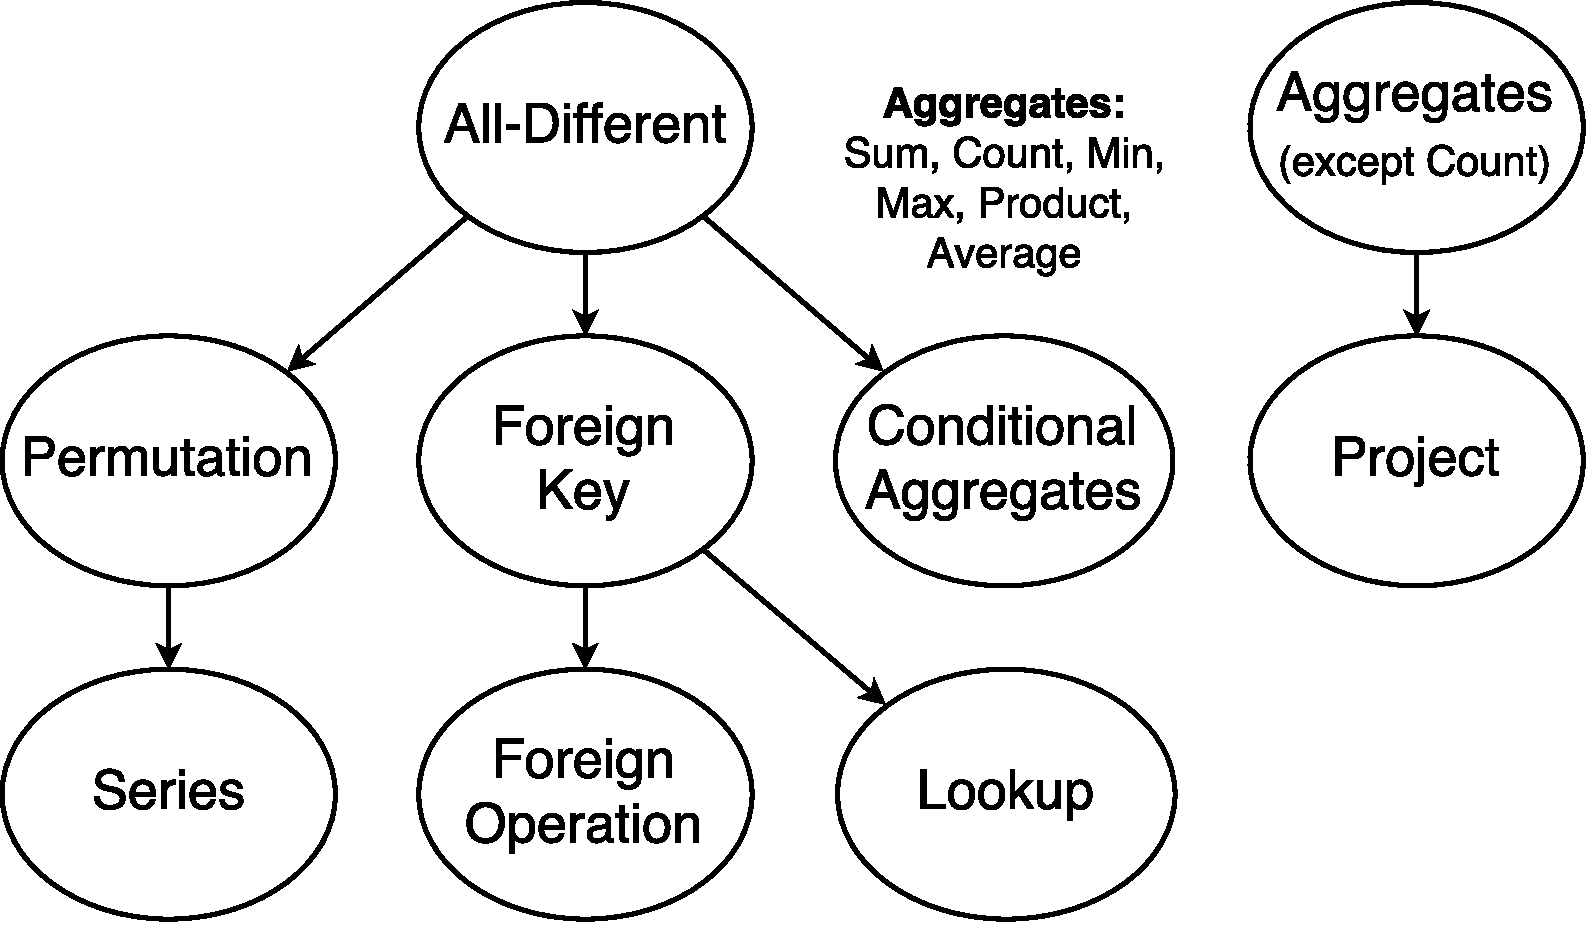
\includegraphics[width=0.8\linewidth]{figures/constraint_dependency2.pdf}
  \caption{Dependency graph; an arrow from~$s_1$ to~$s_2$ indicates that $s_2$ depends on~$s_1$ (the \CSignature of~$s_2$ includes $s_1$).
    The graph is extracted from the Signature column in Table~\ref{table:constraints}.
  }
  \label{fig:learning_order}
\end{figure}

Using the dependency graph~(\dependencies) we can reorder the templates such that a template occurs after any template it depends on.
Concretely, the input templates~$\temps$ (see Algorithm~\ref{algo:tcl}) are reordered to agree with the partial ordering imposed by~\dependencies (e.g. \textit{ALLDIFFERENT} before \textit{FOREIGNKEY}).
Considering Algorithm~\ref{algo:tcl}, this step can be seen as preprocessing the input~\temps.
Learning in this order allows templates to use constraints they depend on, as these constraints will have already been learned.
This is exploited in the \generategroups step to speedup the algorithm by reducing the search space.

\begin{example}
  Consider $\ecfkey{B_{fk}}{B_{pk}}$ whose signature includes $\ecalldiff{B_{pk}}$ and assume that~$C$ are the constraints found for \textit{ALLDIFFERENT}.
  Instead of generating assignments for~$B_{pk}$ using the given blocks~$\blocks$, we will only consider (sub)blocks~$P = \{ B' | \ecalldiff{B'} \in C \}$.
  $P$~can be seen as a set of partial assignments in which the argument $B_{pk}$ has been fixed.
\end{example}

The \generategroups implementation now takes into account previously found constraints to obtain partial assignments~$P$ for a template.
Instead of generating one CSP to find all assignments, a CSP is generated for every~$p \in P$ which finds all assignments completing~$p$.
The procedure to generate CSPs remains the same, except that the partial assignment is used to fix the domains of the dependent variables.

This approach has the additional benefit of ensuring that the (sub)blocks assigned to the dependent arguments already satisfy both the signature and definition of the original template.
Therefore, the implementation of $\findassignment$ does not have to take these blocks into account.





%\subsubsection{Constraint solvers}
%\samuel{Tias, Sergey, have a look at his section, I'm torn about rewriting it, feeling it should either be reduced or expanded, especially the second part.}
%Generic constraint solving technology can be used for the candidate group generation as well as for enumerating the satisfying subgroups.
%Constraint solvers can be categorized as being stand-alone solvers, meaning that they have a text-based modeling language in which the CSP must be formulated, and \textit{embedded}, meaning that they have a programmatic API to formulate the CSP.
%
%\sname supports the ASP \cite{whaisasp} formalism, using the stand-alone Clingo 4.5.4 \cite{clingo} solver, the MiniZinc language \cite{minizinc} with the stand-alone Gecode 4.4.0 solver (which supports floats) and uses an embedded Python-based CP solver \cite{python_constraint}.
%The constraint signature that must be satisfied to generate the groups can be specified in each of the tree formalisms, to ease prototyping and extendability towards new constraints. The embedded solver is fastest as it does not have the overhead of file-writing and calling an external program, and is used in the experiments below.





\subsubsection{Redundancy}
We consider two types of redundancy that we aim to eliminate during the search.
As noted in Section~\ref{sec:form:dependencies}, for some constraint templates there are \textit{symmetries} over the arguments that lead to trivially equivalent solutions, for example, $\ecprod{B_R'}{B_1'}{B_2'} \Leftrightarrow \ecprod{B_R'}{B_2'}{B_1'}$.
Such duplicates are avoided by defining a \textit{canonical} form for these constraints.
In practice, we define an arbitrary but fixed block ordering and require those blocks that are interchangeable to adhere to this ordering.
Moreover, \sname currently contains only product (\ecprod{B_R'}{B_1'}{B_2'}) and not division (\eccalc{B_1'}{B_R' / B_2'}) as well as difference (\ecdiff{B_r}{B_1}{B_2}) and not sum (\eccalc{B_1}{B_r + B_2}).
These choices are based on the prevalence of product and difference in financial spreadsheet data, however, division and sum as well as other constraints could easily be added.


A last type of redundancy we aim to reduce is that there may be multiple \textit{overlapping} subblocks that satisfy the definition of a constraint template.
For example, consider the constraint \ecsumc{B_r}{B[1{:}n]} where $B[k{:}n]$ consists of only zeros, then \ecsumc{B_r}{B[1{:}j]} will be true for all $k - 1 \leq j \leq n$.
In \sname we have, therefore, chosen to only consider \textit{maximal} subblocks.

As a result, in some cases a maximal subblock might falsely include irrelevant columns.
Consider $B_1 = [[200, 300], [200, 150], [1, 2]]$ and $B_2 = [200, 300]$, then \sname will find the constraint $\eccalc{B_2[1]}{\mathit{MAX}(B_1[1{:}3])}$.
Should the target constraint be $\eccalc{B_2}{\mathit{MAX}(B_1[1{:}2])}$, then the last vector of~$B_1$ must be split off into a separate block before the above approach can find it.

Alternatively, we can output all valid argument assignments instead of only maximal subblocks, e.g. $\eccalc{B_2[1]}{\mathit{MAX}(B_1[1])}$, $\eccalc{B_2[1]}{\mathit{MAX}(B_1[1{:}2])}$ and $\eccalc{B_2[1]}{\mathit{MAX}(B_1[1{:}3])}$, however, this might produce many redundant constraints and introduce constraints that accidentally cover too little data.





\subsubsection{Constraints}
The constraints that are currently supported in our system are shown in Table~\ref{table:constraints}.
We included most formulas that we encountered in tutorial spreadsheets including the popular \textit{SUM} and \textit{LOOKUP} constraints\footnote{\href{https://support.office.com/en-us/article/Excel-functions-by-category-5F91F4E9-7B42-46D2-9BD1-63F26A86C0EB}{https://support.office.com/en-us/article/Excel-functions-by-category-5F91F4E9-7B42-46D2-9BD1-63F26A86C0EB}}.
We also added three structural constraints (\textit{ALLDIFFERENT}, \textit{PERMUTATION} and \textit{FOREIGNKEY}) so that they can be used in the signature of other constraint templates; they are also popular in constraint satisfaction~\cite{modelseeker}.

%Their dependencies are reflected in their \CSignature and shown in Figure~\ref{fig:learning_order}.
%These constraints have been selected based on the most-used Excel functions as well as their occurrence in various example spreadsheets we observed.

%Note that \samuel{Motivate why product, not sum (=diff) you only need one, hardcoded preference for display - diff not present - pruning relation?}

% Extending the system with a new constraint template amounts to \tias{TODO: samuel, explain how to define syntax; signature-for-groupgen; signature-for-def; definition}

% \sergey{under question now, might worth deleting} \\
% \sergey{example new template: vr = floor(v), float(v), int(vr), len(v)=len(vr), v,vr are single vectors?}

% \begin{equation}
%   \forall i{:}~ v_r[i] \leq v[i] < v_r[i] + 0.5
%   \label{eq:floor_extension}
% \end{equation}


% \subsection{Workflow}
% \begin{algorithm}[thb]
%   \begin{algorithmic}
%     \footnotesize
%     \State \textbf{Input:} $D$ -- dataset, \constraints -- constraints, \dependencies -- dependencies \\(optional: tables $T$, groups $G$)
%     \State \textbf{Output:} $S$ -- learned constraints with their satisfaction assignment
%     \If{$T$ is \textbf{not} provided}
%       \State $T \gets \extracttables(D)$
%     \EndIf
%     \If{$G$ is \textbf{not} provided}
%       \State $G \gets \extractgroups(D, T)$
%     \EndIf
%     \State $S \gets \learnconstraints(G,\constraints,\dependencies)$
%     \State \Return $S$
% \end{algorithmic}
% \caption{Workflow}
% \label{algo:workflow}
% \end{algorithm}

% \textbf{Approach}
% \begin{itemize}
%   \item Notation
%   \item Algorithm (select constraints, find assignments, find solutions)
% \end{itemize}

% \samuel{Move next to subgroup satisfaction search}
% \section{Declarative modeling}
% \sergey{We need to fit ASP, Minizinc and all that here, I mean it is supposed to be an important point after all}

\newcommand{\runtotal}{16.12}
\newcommand{\runtotalstd}{0.62}

\newcommand{\runfile}{0.50}
\newcommand{\runfilestd}{0.02}

\newcommand{\benchsize}{??}

\section{Evaluation}\label{sec:evaluation}
\sergey{we need to add a summary of the dataset, avg number of constraints, cells, rows, columns}
In this section we experimentally validate our approach.
We studied three main questions concerning the accuracy (\textit{Q1}), precision (\textit{Q2}) and speed (\textit{Q3}) of our algorithm.

The implementation is illustrated using a case study on the spreadsheet corresponding to the previously introduced example (Figure~\ref{fig:main_example}).
In order to quantify the results and generalize our findings we also evaluate our algorithm on a benchmark of 30 (\samuel{check number}) spreadsheets that we assembled from various sources.

There are three main categories of spreadsheets in the benchmark: spreadsheets from an exercise session teaching Excel \samuel{Including running example?}, spreadsheets from tutorials online and publicly available spreadsheets such as crime statistics or financial reports that demonstrate more real world usage\footnote{(attached to to the submitted paper)}.

In this section we focus on \textit{functional} constraints that could be used in spreadsheets, ignoring the structural constraints \textit{ALLDIFFERENT}, \textit{FOREIGNKEY} and \textit{PERMUTATION}.
All experiments were run using Python 3.5.1 (custom Anaconda environment) on a Macbook Pro, Intel Core i7 2.3~GHz with 16GB RAM.






\subsection{Case study}
Let us illustrate our implementation using the example presented in Figure~\ref{fig:main_example}.
\sname takes a few seconds to find the constraints in Figure~\ref{fig:sol_example} (excluding structural constraints).
These include 5 spurious $\mathit{RANK}$ constraints, such as $\ecrank{\range{T_1}{\rangeall}{1}}{\range{T_1}{\rangeall}{5}}$, that are true by accident.
Moreover, there is 1 \textit{LOOKUP} constraint that was not present in the original spreadsheet (looking up ID based on Salesperson).

For this example our primary goal of finding all original constraints is achieved, the recall is $1.0$.
The implementation also returns 6 additional constraints, therefore, our precision is $12/18 = 0.67$, which is rather low compared to other spreadsheets in the benchmark.
The low precision can be explained by the many short vectors which increases the chance for constraints to be true by accident.






\subsection{Benchmark}
All spreadsheets have been converted to CSV files.
Definitions of tables are given (in some harder cases with $\mathit{None}$ values, blocks are defined manually). \samuel{chec}

\samuel{Revisit [what does "implemented" mean here? what's the difference between "implemented" and "algorithm", esp given that we are talking experiments? ] }
\luc{what is not implemented, strange \dots in a paper !!!}
For every spreadsheet a ground-truth has been provided manually, specifying the \textbf{relevant} constraints that are expected to be (re-)discovered.
Not all relevant constraints are currently supported by \sname, therefore, we sometimes consider the subset of \textbf{supported} constraints.
Constraints that are currently outside of the scope of this system, e.g. generic nested mathematical or logical formulas, are ignored.





\subsubsection*{Q1. How accurate is \sname?}
Our implementation achieves a recall of~$0.97$ for relevant constraints, i.e. it finds~90 of~93 relevant constraints in the benchmark suite.
The recall for supported constraints is $1.0$ (90 of 90).





\subsubsection*{Q2. How precise is \sname?}
Our implementation finds 121 constraints across all spreadsheets, 28 of which are not present in the ground-truth.
Therefore, the calculated precision is \samuel{Check numbers}.
Notable, the average precision per spreadsheet is \samuel{math}.
This gap is explained by the large number of additional constraints produced by few spreadsheets \samuel{More info?}.

Examining the additional constraints more closely reveals that only \samuel{x} of the constraints are spurious, i.e. they hold by accident and can be disproved by adding additional data.
Most constraints are \textit{redundant}, such as duplications or implications of other constraints.
Many redundant constraints are the result of bad spreadsheet design, i.e. copying data in multiple places, and the overlapping role of difference and the sum aggregate.

We consider precision (i.e. avoiding redundant constraints) a secondary goal, focusing primarily on accuracy.
The rationale is that the precision can be increased by post-processing the constraints using entailment or heuristics.





\subsubsection*{Q3. How fast is \sname?}
Concerning the speed of the algorithm we also prioritized accuracy when a trade-off had to be made.
For the \benchsize~spreadsheets in the benchmark our implementation ran in ${\runtotal}s \pm {\runtotalstd}s$.
The execution times vary widely though between spreadsheets, only four spreadsheets taking more than $0.2s$.
Most of the execution time in these cases goes towards searching either aggregate constraints or conditional aggregates.
The search for aggregates will be slow on spreadsheets containing larger groups of numeric data.
For conditional aggregates the number of candidate primary keys (all-different) and numeric vectors determines the running time (e.g. the case study example).

\begin{table}
  \caption{Overview evaluation on benchmark}
  \centering
  \begin{tabular}{lll}
    & \textbf{Total} & \textbf{Spreadsheet (avg)} \\
    \textbf{Relevant constraints} & $93$ & $2.91$ \\
    \textbf{Recall} & $96.77\%$ & $94.27\%$ \\
    \textbf{Precision} & $23.14\%~(28)$ & $8.33\%~(0.88)$ \\
    \textbf{Speed (s)} & ${\runtotal}s \pm {\runtotalstd}s$ & ${\runfile}s \pm {\runfilestd}s$
  \end{tabular}
\end{table}
\samuel{Expand summary}
\sergey{would it make sense to specify the size of a spreadsheet in the number of non-zero cells?}

We explained various optimizations, most notably the exploitation of dependencies.
Using the dependencies to find constraints incrementally cuts down large parts of the search trees, especially for constraints that have many arguments.
Essentially, one obtains a more specialized search without much effort.


In order for the algorithm to run efficiently it is crucial to use dependencies and find constraints incrementally whenever possible.
This avoids some of the explosion of combinations for constraints that have many arguments.
For example, using foreign keys as a base constraint to find conditional aggregates reduces the running time for the case study from about 3 seconds to below 1 second.
Unfortunately, this assumption is sometimes too strong, when users are interested in aggregates for only some of the keys that are present in the data.





\section{Applications}\label{sec:applications}
In this section, we illustrate how various motivating applications could be realized using our system.





\subsection{Autocompletion}
Autocompletion can be seen as using knowledge derived from a snapshot of spreadsheet data to predict new values before they are written by the user.
The snapshot~($D_0$) is used to learn constraints and these are combined with new data~($\Delta D$) that the user has added.
Using~$\Delta D$ we can keep track of which vectors have changed and which vectors are now incomplete.
A \textit{functional} constraint corresponds to a spreadsheet formula.
Such a constraint, e.g. $\ecsumc{B_r}{\mathbf{B_x}}$, is able to compute a result~($B_r$) based on its input~($\mathbf{B_x}$).
If all the input vectors / blocks have been filled and the result is incomplete, the constraint can predict the result value(s).

Let us illustrate this on one of the spreadsheets from the gathered dataset.
Consider Figure \ref{fig:autocompletion_example} containing two tables.
By learning constraints on the tables excluding the last row, we find constraints $\ecsumif{\range{T_2}{\rangeall}{2}}{\range{T_1}{\rangeall}{2}}{\range{T_2}{\rangeall}{1}}{\range{T_1}{\rangeall}{3}}$ and $\ecsumif{\range{T_2}{\rangeall}{3}}{\range{T_1}{\rangeall}{2}}{\range{T_2}{\rangeall}{1}}{\range{T_1}{\rangeall}{4}}$.
The new data $\Delta D$ consists of the new value \textit{West} in the last row.
Therefore, vector~$\range{T_2}{:}{1}$ is changed and vectors~$\range{T_2}{:}{2}$, $\range{T_2}{:}{3}$ have become incomplete.
The \textit{SUMIF} constraints have enough input to fill the incomplete vectors and predict the values in the last row: $\range{T_2}{4}{2} = 1547$ and $\range{T_2}{4}{3} = 428128$.

In case multiple constraints predict different values for the same cell, the algorithm will have to either prioritize constraints based on their specificity or a heuristic, not make a prediction, or present the choice to the user.

\subsection{Error detection}
\begin{figure*}[thb]
\begin{subfigure}{.70\textwidth}
  \begin{center}
    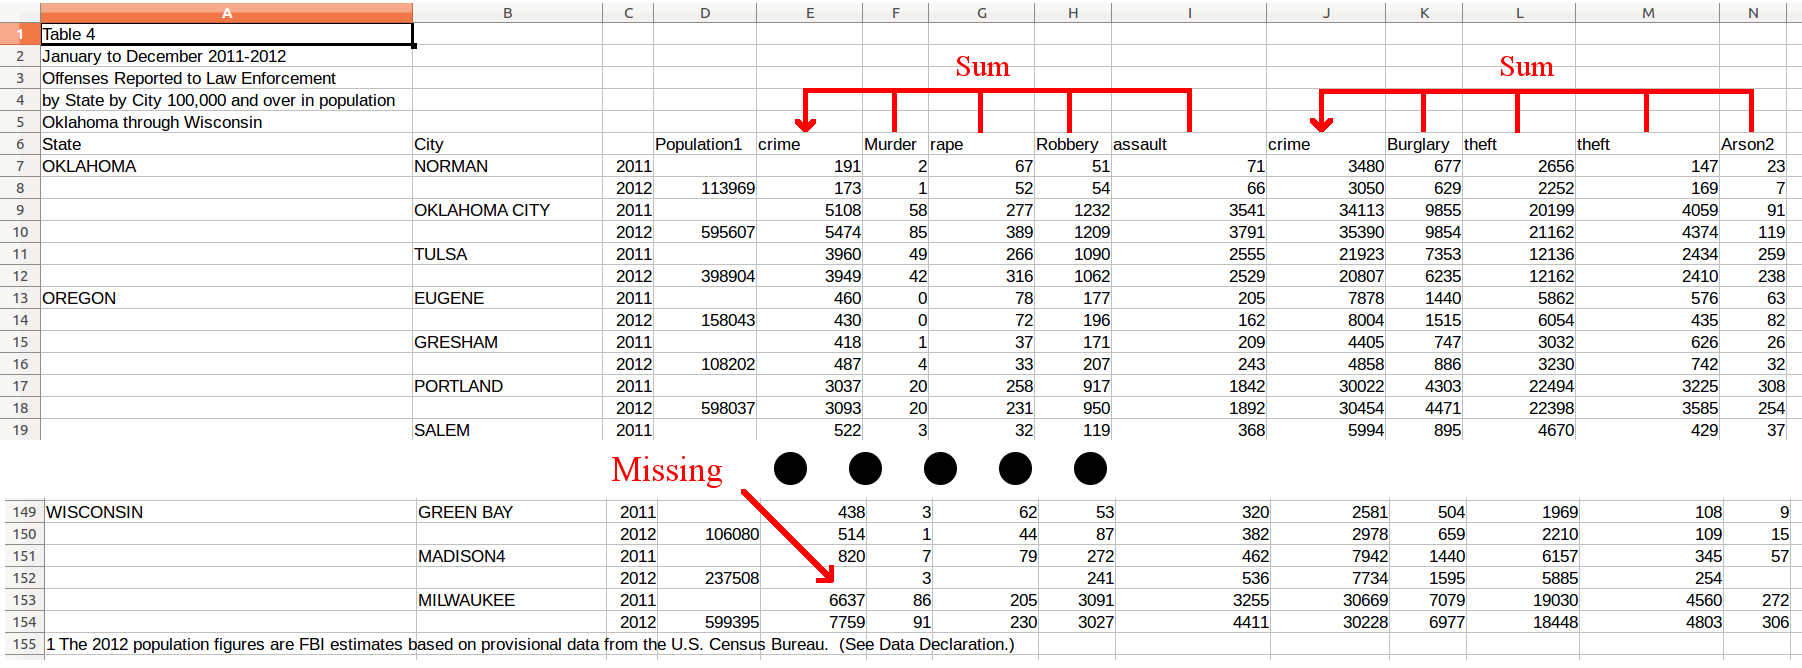
\includegraphics[width=\textwidth]{figures/fbi_figure_highlighted.png}
  \end{center}
  \caption{Real world tabular constraint reconstruction: FBI crime statistics}
  \label{fig:fbi}
\end{subfigure}
\hfill
\begin{subfigure}{.29\textwidth}
\begin{center}
    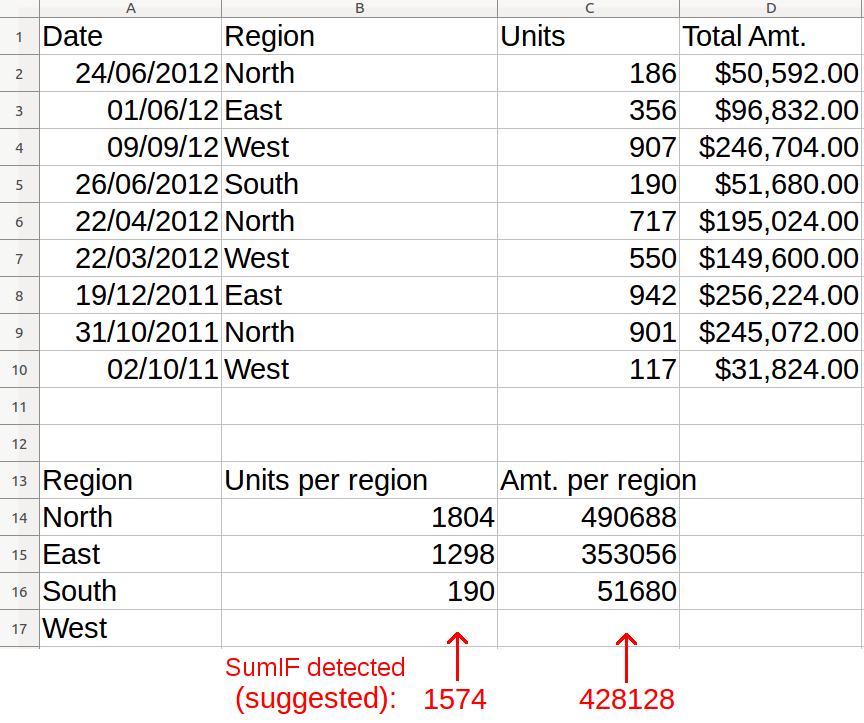
\includegraphics[width=\textwidth]{figures/autocompletion_example.png}
  \end{center}
  \caption{\sergey{Samuel, Tias have a look at it, should be corrected and extended, like with groups indications and formulas?}}
  \label{fig:autocompletion_example}
\end{subfigure}
\end{figure*}

We consider two cases of error detection.
The first setting is the \textit{online} detection of errors which is similar to the autocompletion setting.
However, we look at \textit{conflict} constraints, i.e. constraints that were learned on the snapshot data but do not agree with the newly added data~$\Delta D$.
Such conflict constraints can indicate errors in the input.
However, such conflicts can be wrongly caused by spurious constraints.
Therefore, conflicts should only be detected if the snapshot data is large enough. An exact specification of what large enough means (i.e., how to measure the confidence in the constraint violation) is a separate application-dependent research question and will be investigated in the future work.

The second type of error detection is \textit{offline} and attempts to detect errors in a spreadsheet.
Consider, for example, a use case concerning crime statistics provided by the FBI.
An extract of the spreadsheet is depicted in Figure~\ref{fig:fbi}.
When run on this sheet, our system is able to detect the second sum constraint, however, a missing value prevents the first sum constraint from being learned.
A possible approach to detect such missing or wrong values is to look at a sample of the table that excludes the erroneous row, e.g. trying to leave out each row, and compare the constraints learned on this sample with the constraints learned by adding the row containing the mistake.
The sample needs to be large enough such that we have enough confidence that the constraints are correct. For example, in Figure \ref{fig:fbi} all but one row satisfy the constraint, which is a strong indication that there is a constraint violation.
If we define the sample to be the snapshot data and the added row to be the additional input~$\Delta D$, this task can be formulated as online error detection and dealt with in the same way.
%Of course, generating large enough samples and rows (columns) to be added can be done in multiple ways.
%In the limited case of detecting single errors one can leave out every row (column), consider the remaining data to be the sample and
%and the left out row (column) to be new input.

\section{Related Work}\label{sec:related_work}
\sname combines ideas from several existing
approaches from multiple different fields of research.


First, it borrows techniques from logical and relational learning \cite{luc_book}, as it finds
constraints in multiple relations (or tables). However, unlike typical logical and relational learning
approaches, it focuses on data in spreadsheets and on constraints that can be column or row-wise.
Furthermore, it derives a set of simple “atomic” constraints rather than a set of rules that each consist of multiple literals as in clausal discovery \cite{claudien,lallouet}. Still several ideas from logical and relational learning
proved to be useful, such as the use of a canonical form, a refinement graph, and pruning for redundancy.
Also related to this line of research is the work on deriving constraints in databases such as functional and multi-valued dependencies \cite{savnik, Mannila-Raiha}
although this line of research has focused on more specialized techniques for specific types of constraints. Furthermore, the constraints used
in spreadsheets are often quite different than those in databases.


Second, there exist several algorithms in the constraint programming community that induce constraint (programs)
from one or more examples and questions. Two well-known lines of research include ModelSeeker \cite{modelseeker} and Quacq \cite{Quacq}.
The former starts from a single example in the form of a vector of values and then exhaustively looks for the most specific constraints from a large constraint library that hold in the vector. To this aim, it cleverly enumerates different tables from the vector. For instance, if the initial vector was of dimension $1 \times 20$, it would consider rearrangements of size $2 \times 10$, $4 \times 5$, $5 \times 4$, … and Modelseeker would then look for both column, row  and even diagonal constraints. Key differences with our technique are that we assume the tables are given (a reasonable assumption if one starts from a spreadsheet), and also that ModelSeeker’s constraints are the typical ones from the constraint programming community\tias{which is all over integers, we also over strings and real-valued, AND, not one vector but we have many indep. blocks}, which are aimed at combinatorial optimization and scheduling rather than what is typically used in spreadsheets. Quacq \cite{Quacq} and its predecessor Conacq \cite{Conacq} acquire a conjunction of constraints using techniques inspired on Mitchell's version spaces to process examples, some variants also asking informative questions to the user. As the conjunction for typical constraint programming problems (such as Sudoku) can be quite large, a key problem is to cope with redundant constraints\tias{it looks only at pairwise constraints, so an important factor is how fast the algorithm can converget to the entire constraint set. Redundant and spur also issue for these methods}. As Modelseeker, these systems focus on the types of constraints in combinatorial optimization but unlike ModelSeeker and our approach, they do not assume the variables are organized in tabular form.


Third, our work borrows from the seminal work of Gulwani et al. \cite{flashfill} on program synthesis for tabular data that is incorporated in Microsoft’s Excel. In FlashFill, the end-user might work on a table containing the surnames (column A) and names (column B) of politicians. The first row might contain the values A1 = ``Blair'' and B1 = ``Tony'', and the user might then enter in cell C1 the value ``T.B.''. At that point FlashFill would generate a program that produces the output ``T.B.'' for the inputs ``Blair'' and ``Tony'', would also apply it to automatically generate values for the other politicians (rows) in the table. While it might need an extra example to deal with names such as ``Van Rompuy, Herman'' and determine whether it should output ``H.V.'' or ``H.V.R.'', FlashFill learns correct programs from very few examples. Flashfill has been extended to e.g. FlashExtract \cite{flashextract} to produce a set of tables starting from a document (a txt, spreadsheet or HTML file) with a set of examples marked for extraction. However, unlike our approach, Flashfill requires the user to identify explicitly the desired inputs/outputs from the function as well as to provide explicitly some positive and sometimes also negative examples.  In contrast, our approach is unsupervised, although it would be interesting to study whether it could be improved through user interaction and through user examples.  Another interesting open issue (for all of these techniques with the exception of logical and relational learning) is how to deal with possibly incomplete or noisy data.

Finally, there are the works on  BayesDB \cite{BayesDB} and Tabular \cite{tabular}, two recent probabilistic modeling languages that have been specifically designed for dealing with relational data in tabular form and that can, as FlashFill, also automatically fill out missing values in a table.  However, unlike the other mentioned approaches, it is based on an underlying probabilistic graphical model that performs probabilistic inference rather than identify ``hard'' constraints.

\section{Conclusions}\label{sec:conclusions}

% points: 1) can be a base for an actual plugin or a function in excel 2) novel problem and challenge for systems and constraint solvers 3) can be part of the complicated pipeline togehter with the header detection
Our goal is to automatically identify constraints in a spreadsheet.
We have presented and evaluated our approach, implemented as the system \sname, that is able to learn a large set of constraints from CSV data.
Moreover, the amount of redundant constraints found by the system is limited despite the lack of more sophisticated post-processing steps.

For the future development of the system there are multiple directions. Integrating the system in an interactive setting would offer users the possibility to easily receive and provide feedback.
Moreover, the system can be adapted to deal with additional types and produce less redundant constraints through the use of (heuristic) filtering or post-processing.

Currently, the system only learns single constraints and extending our approach to nested constraints would allow more expressive concepts to be learned. Also, \sname only works on complete rows and columns, allowing partial vectors is an important future direction for developing applications based on the system.
%This shift would bring the approach in line with programming by example.

Aside from finding errors, the system can be extended to deal with noise and the ability to learn soft constraints.
Soft constraints are (potentially weighted) constraints that hold only on some of the data.
This would extend the approach to new application domains as well as provide more native error detection.


\bibliographystyle{plain}
{\footnotesize
  \bibliography{references}}
\end{document}
%%%%%%%%%%%%%%%%%%%%%%%%%%%%%%%%%%%%%%%%%%%%%%%%%%%%%%%%%%%%%%%%%%%%%%
